% !TeX program = xelatex
\documentclass[twoside]{article}
\usepackage{amsmath}
\usepackage{amssymb}
\usepackage{amsthm}
\usepackage{graphicx}
\usepackage{wasysym}
\usepackage{mathspec}
\usepackage{calc}
\setmainfont[Path=../fonts/,BoldFont={Futura_Heavy.ttf},ItalicFont={Futura_Medium_Italic.ttf},BoldItalicFont={Futura_Bold_Italic.ttf}]{Futura_Medium.ttf}
\setmathfont[Path=../fonts/]{Futura_Book.ttf}
\setmathrm[Path=../fonts/]{Futura_Book.ttf}
\newfontfamily\myfonta[Path=../fonts/]{Friz_Quadrata_Bold.otf}
\newfontfamily\myfontb[Path=../fonts/]{Korinna_Bold.ttf}
\usepackage[inner=0.7in,outer=0.3in,top=0.3in,bottom=0.5in]{geometry}
\usepackage{moresize}
\usepackage{adjustbox}
\usepackage{hyperref}
\usepackage[capitalize]{cleveref}
\usepackage{multirow}
\usepackage{booktabs}
\usepackage{colortbl}
\usepackage{hhline}
\usepackage{titlesec}
\titleformat*{\section}{\large\bfseries}
\titleformat*{\subsection}{\bfseries}
\titleformat*{\subsubsection}{\bfseries}
\titleformat*{\paragraph}{\bfseries}
\titleformat*{\subparagraph}{\bfseries}
\usepackage[titles]{tocloft}
\renewcommand{\contentsname}{\hfill\large CONTENTS\hfill}   
\renewcommand{\cftaftertoctitle}{\hfill}
\renewcommand{\cftsecleader}{\cftdotfill{\cftdotsep}}
\setlength{\cftbeforesecskip}{0pt}
\renewcommand\cftsecfont{\mdseries}
\renewcommand\cftsecpagefont{\mdseries}
\usepackage{parskip}
\usepackage{caption}
\captionsetup{singlelinecheck=false,justification=raggedright,font={bf},tablename=TABLE,hypcap=false}
\renewcommand{\thetable}{\Roman{table}.}
\usepackage{faktor}
\usepackage{enumitem}

\newcommand{\TTN}[2]{\textbf{Thread the Needle} above #1 and below #2}
\newcommand{\lle}{\raisebox{\depth}{\rotatebox{180}{$\ell$}}}
\newcommand{\mysection}[1]{\phantomsection\section*{#1}\addcontentsline{toc}{section}{#1}}
\newcommand{\mysubsection}[1]{\phantomsection\subsection*{#1}\addcontentsline{toc}{subsection}{#1}}
\newcommand{\tableandchartline}[1]{\nameref{#1}\dotfill\pageref*{#1}}
\newcommand{\boldref}[1]{\textbf{\hyperref[#1]{\cref{#1}}}}   

%\usepackage{showframe}
\begin{document}
\begin{titlepage}
\newgeometry{left=0in,right=0in,top=0.3in,bottom=0.5in}
\centering

\phantom{x}

\vspace{1in}

{\myfonta\raisebox{1ex}{\large \phantom{Official}} \HUGE{\phantom{Advanced}\\Gold \& Gallows}}

\vspace{3ex}

{\myfontb\HUGE{RULES BOOKLET}}
\end{titlepage}
\pagebreak

\restoregeometry
\begin{center}
\tableofcontents

\bigbreak

\large\textbf{TABLES AND CHARTS}\normalsize

\begin{tabular}[t]{>{\centering\arraybackslash}p{0.5\columnwidth -2\tabcolsep}>{\centering\arraybackslash}p{0.5\columnwidth -2\tabcolsep}}
\tableandchartline{gear}&\tableandchartline{morale}\\
\tableandchartline{armor}&\tableandchartline{magicuserav}\\
\tableandchartline{classes}&\tableandchartline{magicuserspells}\\
\tableandchartline{clericav}&\tableandchartline{monster}\\
\tableandchartline{clericspells}&\tableandchartline{paladinav}\\
\tableandchartline{consumable}&\tableandchartline{paladinspells}\\
\tableandchartline{druidav}&\tableandchartline{property}\\
\tableandchartline{druidspells}&\tableandchartline{rangerav}\\
\tableandchartline{dwarfav}&\tableandchartline{rangerspells}\\
\tableandchartline{elfav}&\tableandchartline{warlockav}\\
\tableandchartline{elfspells}&\tableandchartline{warlockspells}\\
\tableandchartline{fighterav}&\tableandchartline{level}\\
\tableandchartline{halflingav}&\tableandchartline{weapons}\\
\tableandchartline{hirelings}\\
\end{tabular}
\end{center}

\twocolumn

\mysection{INTRODUCTION}

\textbf{GOLD \& GALLOWS} is a pen and paper tabletop roleplaying game - an homage to the world's most popular fantasy roleplaying game. It has been designed to be mathless and streamlined while still retaining compatibility with its inspiration and the wide variety of old school supplemental materials that exist.

\bigbreak

To play, all you need is the standard role playing dice, nonstandard Zocchi dice if playing a Warlock, character sheets, and if so desired, miniatures for fictional positioning.

\bigbreak

The core mechanic in \textbf{GOLD \& GALLOWS} involves rolling a d20. In an unopposed check, a player must roll \emph{strictly below} their relevant stat to succeed. If the check is opposed, then the player must \textbf{Thread the Needle}; they must roll a d20 that lands simultaneously \emph{strictly below} their relevant stat and \emph{strictly above} an opposing value. Throughout this book, this is denoted with the instructions to ``\TTN{\{lower bound\}}{\{upper bound\}}." 

\mysection{CHARACTER CREATION}

\mysubsection{Roll Stats}

Every character has six stats: \emph{Charisma} (CHA), \emph{Constitution} (CON), \emph{Dexterity} (DEX), \emph{Intelligence} (INT), \emph{Strength} (STR), and \emph{Wisdom} (WIS). To assign stats when creating a character, roll dice six times and assign the results to your stats in the order above. Ask your Referee which of the following you will use:

\bigbreak

\textbf{EXTREME}: Roll 3d20 and take the highest. This results in an average stat of about 15.5. Use this for overpowered PCs in heroic campaigns.

\textbf{STANDARD}: Roll 3d10 and add the highest two. This results in an average stat of about 13.5. Use this for campaigns where the PCs are remarkable people but not necessarily superhuman.

\textbf{CLASSIC}: Roll 3d6 and add all three. This results in an average stat of 10.5. Use this for PCs beginning of comparable power to any average schmuck in the world.

\mysubsection{Choose a Class}

A class is a character's specialization or role in the group. There are ten classes: \emph{Cleric}, \emph{Druid}, \emph{Dwarf}, \emph{Elf}, \emph{Fighter}, \emph{Halfling}, \emph{Magic-User}, \emph{Paladin}, \emph{Ranger}, and \emph{Warlock}. The character's class determines their Health Points (HP), Attack Value (AV) progression, permissible weapon damage dice, and abilities.

\mysubsection{Purchase Equipment}

Every character begins with 3d6$\times$10 gold, clothes, and a free weapon as permitted by their class. The number of items a character can carry is their STR score.

\bigbreak

The items listed in \textbf{EQUIPMENT} are not intended to be an exhaustive list of every item that can be purchased or sold.

\mysubsection{Leveling Up}

Characters level up by spending (not necessarily all at once) the amount of gold listed on \boldref{level}. Upon level up, you gain abilites and HP based on your class. You can also attempt to improve your stats. Pick a stat and roll a d20; if you roll higher than your score, you can increase that stat by 1. If you roll lower, you can try another stat, but note you can only increase at most three stats each time you level up.

\bigbreak

\begin{center}
\captionof{table}{WEALTH REQUIRED TO SPEND TO LEVEL UP.}\label{level}
\noindent\begin{tabular}{>{\centering\arraybackslash}p{.5\columnwidth -2\tabcolsep}>{\centering\arraybackslash}p{.5\columnwidth -2\tabcolsep}}
\textbf{Level}&\textbf{Cost}\\
\rowcolor[gray]{0.75}2&{\leavevmode\phantom{001,}500 gold}\\
\rowcolor[gray]{0.75}3&{\leavevmode\phantom{00}1,000 gold}\\
\rowcolor[gray]{0.75}4&{\leavevmode\phantom{00}2,000 gold}\\
5&{\leavevmode\phantom{00}4,000 gold}\\
6&{\leavevmode\phantom{00}8,000 gold}\\
7&{\leavevmode\phantom{0}16,000 gold}\\
\rowcolor[gray]{0.75}8&{\leavevmode\phantom{0}32,000 gold}\\
\rowcolor[gray]{0.75}9&{\leavevmode\phantom{0}64,000 gold}\\
\rowcolor[gray]{0.75}10&128,000 gold\\
\end{tabular}
\end{center}

%\bigbreak

\mysection{EQUIPMENT}

Weapons are classified into three different groups based on the amount of damage they deal. The three groups are d8, d6, and d4. Any melee weapon can belong to any damage category. Ranged weapons can deal at most d6 damage.

\bigbreak

\begin{center}
\captionof{table}{WEAPONS.}\label{weapons}
\noindent\begin{tabular}{>{\centering\arraybackslash}p{.5\columnwidth -2\tabcolsep}>{\centering\arraybackslash}p{.5\columnwidth -2\tabcolsep}}
\textbf{Type}&\textbf{Cost}\\
\rowcolor[gray]{0.75}d8&100 gold\\
d6&{\leavevmode\phantom{0}60 gold}\\
\rowcolor[gray]{0.75}d4&{\leavevmode\phantom{0}40 gold}\\
\end{tabular}
\end{center}

\bigbreak

Armor is also classified into three groups: light, medium, and heavy. The groups give a +1, +2, or +3 bonus, respectively, to checks to evade monster attacks. Shields are small (+1) or large (+2). A character's Armor Class (AC) is their DEX score + any bonus from armor and shields. Choice of class may restrict which armor and shields you may use.

\bigbreak

\begin{center}
\captionof{table}{ARMOR AND SHIELDS.}\label{armor}
\noindent\begin{tabular}{p{.8\columnwidth -2\tabcolsep}>{\centering\arraybackslash}p{.2\columnwidth -2\tabcolsep}}
\centering\textbf{Type}&\textbf{Cost}\\
\rowcolor[gray]{0.75}Light armor (+1), e.g., hides and leathers&{\leavevmode\phantom{0}50 gold}\\
Medium (+2), e.g., chain mail&300 gold\\
\rowcolor[gray]{0.75}Heavy (+3), e.g., plate&600 gold\\
Small shield (+1)&{\leavevmode\phantom{0}50 gold}\\
\rowcolor[gray]{0.75}Large (+2)&100 gold\\
\end{tabular}
\end{center}

\bigbreak

Consumable items have a usage die. When you use an item, roll the corresponding usage die. If the result is a 1 or 2, the usage die is downgraded to the next lowest die: d20>d12>d10>d8>d6>d4. A roll of 1 or 2 on a d4 expends the consumable item. If no usage die is listed, the item has a single use.

\bigbreak

\begin{center}
\captionof{table}{CONSUMABLE ITEMS.}\label{consumable}
\noindent\begin{tabular}{p{.5\columnwidth -2\tabcolsep}>{\centering\arraybackslash}p{.25\columnwidth -2\tabcolsep}>{\centering\arraybackslash}p{.25\columnwidth -2\tabcolsep}}
\textbf{Item}&\textbf{Cost}&\textbf{Usage Die}\\
\rowcolor[gray]{0.75}Antipoison&15 gold&-\\
\rowcolor[gray]{0.75}Arrows&10 gold&d10\\
\rowcolor[gray]{0.75}Bandages&{\leavevmode\phantom{0}5 gold}&-\\
Daily rations&{\leavevmode\phantom{0}5 gold}&d4\\
Herbs: poultice, aroma, seasoning&10 gold&d8\\
\rowcolor[gray]{0.75}Oil&{\leavevmode\phantom{0}2 gold}&d6\\
\rowcolor[gray]{0.75}Torch&{\leavevmode\phantom{0}1 gold}&d6\\
\rowcolor[gray]{0.75}Waterskin&{\leavevmode\phantom{0}1 gold}&d6\\
\end{tabular}
\end{center}

\bigbreak

Antipoison can cure or preemptively prevent one bout of poison/toxin. Bandages take time to apply, but heal d4 damage, d6 with poultice. A character that neglects their daily rations becomes Disadvantaged (see \textbf{Advantage and Disadvantage}) in all rolls and eventually dies.

\bigbreak

\begin{center}
\captionof{table}{ADVENTURING GEAR.}\label{gear}
\noindent\begin{tabular}{>{\centering\arraybackslash}p{.5\columnwidth -2\tabcolsep}>{\centering\arraybackslash}p{.5\columnwidth -2\tabcolsep}}
\textbf{Item}&\textbf{Cost}\\
\rowcolor[gray]{0.75}10 foot pole&{\leavevmode\phantom{0}1 gold}\\
\rowcolor[gray]{0.75}10 foot ladder&{\leavevmode\phantom{0}5 gold}\\
\rowcolor[gray]{0.75}50 foot rope&{\leavevmode\phantom{0}1 gold}\\
Bedroll&{\leavevmode\phantom{0}1 gold}\\
Flint \& steel&{\leavevmode\phantom{0}3 gold}\\
Lantern&10 gold\\
\rowcolor[gray]{0.75}Mirror&{\leavevmode\phantom{0}5 gold}\\
\rowcolor[gray]{0.75}Ram&10 gold\\
\rowcolor[gray]{0.75}Sack&{\leavevmode\phantom{0}1 gold}\\
Spikes&{\leavevmode\phantom{0}1 gold}\\
Tent&10 gold\\
Winter blanket&{\leavevmode\phantom{0}1 gold}\\
\end{tabular}
\end{center}

\bigbreak

Characters can employ hirelings to assist them in adventures. Hirelings demand a share of the wealth your character brings safely back to civilization. They are paid once the party arrives in a safe, familiar place. The adventurer is left with whatever wealth remains after dividing it among all their surviving hirelings.

\bigbreak

\begin{center}
\captionof{table}{HIRELINGS.}\label{hirelings}
\noindent\begin{tabular}{>{\centering\arraybackslash}p{.5\columnwidth -2\tabcolsep}>{\centering\arraybackslash}p{.5\columnwidth -2\tabcolsep}}
\textbf{Hireling}&\textbf{Share}\\
\rowcolor[gray]{0.75}Animal handler&10\%\\
\rowcolor[gray]{0.75}Classed hireling&50\%\\
\rowcolor[gray]{0.75}Dungeoneer&15\%\\
Guard&10\%\\
Guide&10\%\\
Lantern bearer&{\leavevmode\phantom{0}8\%}\\
\rowcolor[gray]{0.75}Mercenary&20\%\\
\rowcolor[gray]{0.75}Porter&10\%\\
\rowcolor[gray]{0.75}Servant&{\leavevmode\phantom{0}5\%}\\
\end{tabular}
\end{center}

\bigbreak

A classed hireling is generated like a player character. For a mercenary, assign the stats 12-11-10-10-9-9 in an order you choose, d8 HP, and 9 AV. Assign to all other hirelings the stats 10-10-9-9-9-9 as you choose, d6 HP, and 8 AV. Any equipment a hireling uses must be purchased by their employer. Only classed hirelings can level up.

\bigbreak

Wealthy characters can invest in property. Purchasing the land and/or building is only one step towards maintaining a property. Money must also periodically be invested for maintenance and upkeep as well.

\bigbreak

\begin{center}
\captionof{table}{PROPERTY.}\label{property}
\noindent\begin{tabular}{p{.25\columnwidth -2\tabcolsep}>{\centering\arraybackslash}p{.45\columnwidth -2\tabcolsep}>{\centering\arraybackslash}b{.3\columnwidth -2\tabcolsep}}
\textbf{Property}&\textbf{Purchase Price}&\textbf{Monthly Upkeep Cost}\\
\rowcolor[gray]{0.75}Brewery \& tavern&{\leavevmode\phantom{00,}900 gold}&{\leavevmode\phantom{0,0}75 gold}\\
\rowcolor[gray]{0.75}Castle&{\leavevmode\phantom{0}7,500 gold}&{\leavevmode\phantom{0,}550 gold}\\
Crypt&{\leavevmode\phantom{0}2,000 gold}&{\leavevmode\phantom{0,0}10 gold}\\
Dungeon&{\leavevmode\phantom{0}1,750 gold}&{\leavevmode\phantom{0,0}75 gold}\\
Estate&{\leavevmode\phantom{0}4,000 gold}&{\leavevmode\phantom{0,}800 gold}\\
\rowcolor[gray]{0.75}Farm&{\leavevmode\phantom{0}2,000 gold}&{\leavevmode\phantom{0,}120 gold}\\
\rowcolor[gray]{0.75}Fort&{\leavevmode\phantom{0}6,000 gold}&{\leavevmode\phantom{0,}250 gold}\\
\rowcolor[gray]{0.75}Guild&{\leavevmode\phantom{0}2,750 gold}&{\leavevmode\phantom{0,}175 gold}\\
House&{\leavevmode\phantom{0}1,300 gold}&{\leavevmode\phantom{0,0}25 gold}\\
Mansion&{\leavevmode\phantom{0}5,250 gold}&{\leavevmode\phantom{0,}375 gold}\\
Monument&{\leavevmode\phantom{00,}500 gold}&{\leavevmode\phantom{0,00}5 gold}\\
\rowcolor[gray]{0.75}Palace&25,000 gold&2,500 gold\\
\rowcolor[gray]{0.75}Temple&{\leavevmode\phantom{0}1,500 gold}&{\leavevmode\phantom{0,0}75 gold}\\
\rowcolor[gray]{0.75}Vault&{\leavevmode\phantom{00,}800 gold}&{\leavevmode\phantom{0,0}75 gold}\\
Villa&{\leavevmode\phantom{0}9,000 gold}&1,500 gold\\
Watchtower&{\leavevmode\phantom{0}1,500 gold}&{\leavevmode\phantom{0,0}75 gold}\\
Waterfront&{\leavevmode\phantom{0}2,750 gold}&{\leavevmode\phantom{0,}225 gold}\\
\end{tabular}
\end{center}

\mysection{GAMEPLAY}

During a player's turn, their character may move and act. An action is, generally speaking, any interaction with the world: attacking, casting a spell, searching, talking, and so on. The Referee has final say in what can or cannot be done in a single turn, and some actions take multiple turns. A round is the cumulative total of all characters' turns.

\bigbreak

Explicit tracking of rounds and turns happens during combat and time-sensitive scenarios; outside of these circumstances, characters can act as they please, under Referee direction.

\mysubsection{Movement}

A character can move up to 30 feet in their turn. If they forgo their action, they may move an additional 30 feet.

\mysubsection{Initiative}

When combat is imminent, players roll a check against DEX; i.e., they attempt to roll a d20 under their DEX score. Those successful go before the enemy; those not go after.

\mysubsection{Combat}

If a player is attempting a melee or ranged attack, then they must \TTN{the enemy's Hit Dice (HD)}{the character's AV}. 

\bigbreak

If an enemy attacks a character with melee or ranged, then to defend, the player must \TTN{enemy HD}{the character's AC}. 

\bigbreak

If a melee or ranged attack is successful, then damage is rolled. For a character, damage is rolled based on the weapon they are using. For a monster, damage is rolled based on their HD as described in the \textbf{ADVERSARIES} section.

\bigbreak

If a player is using a spell on an enemy, then they must \TTN{enemy HD}{the class's spellcasting stat (see below)}.

\bigbreak

\textbf{Thread the Needle} with:

CHA if you are a Paladin.

INT if you are an Elf, Magic-User, or Warlock.

WIS if you are a Cleric, Druid, or Ranger.

\bigbreak

If an enemy attacks a character with magic, then the player needs to roll a save for the relevant stat.

\mysubsection{Checks and Saves}

In unopposed checks, a player must simply roll below the stat they are testing. For an opposed check, e.g., to resist a spell, trap, effect, or so on, they \TTN{opposing HD}{the relevant stat}. The Referee will indicate which stat to use based on the following.

\bigbreak

\textbf{Thread the Needle} with:

CHA when the save is against charming effects.

CON when the save is against poison, disease, or death.

DEX when the save is against physical harm that can be dodged.

INT when the save is against spells and magic.

STR when the save is against physical harm that cannot be dodged.

WIS when the save is against deception and illusions.

\mysubsection{Recovery}

Characters can recover lost HP by bandaging their wounds, drinking health potions, casting certain spells, and resting. A character cannot surpass their maximum HP by mundane means.

\mysubsection{Death}

A character that reaches 0 HP is dying. They are unable to move or act in the current combat any longer. After combat has ended, the player must \TTN{the amount of damage under 0 their character has taken}{CON}. If successful, the character is alive at d4 HP and can resume action, but with a scar or disfigurement. If the check fails, the character dies in a comrade's arms, though magic exists to raise the dead, if they had a soul.

\bigbreak

Monsters that reach 0 HP get no such special privileges; they are immediately dead.

\mysubsection{Advantage and Disadvantage}

When the Referee determines that a task is particularly easy or hard given the circumstances, they may ask for a roll at Advantage or Disadvantage. For a roll at Advantage, roll twice; if at least one of the rolls is successful, then you have succeeded. For a roll at Disadvantage, roll twice; both rolls must be successful in order for you to succeed. Advantage and Disadvantage cancel each other in pairs.

\mysubsection{Morale}

When things go south for adventurers, as things so often do, adventurers rarely break under pressure, but hirelings do. In circumstances such as imminent defeat, total darkness, the death of a character, and so on, the Referee may ask players to make a morale check to retain their hirelings. In a morale check, players must \TTN{the hireling's morale score (in \boldref{morale})}{CHA}. If a hireling is particularly well-treated, their morale score may go down, at the discretion of the Referee, and vice versa: poor treatment raises morale score. Each player should roll once; this single roll is the morale check for all their character's hirelings.

\bigbreak

\begin{center}
\captionof{table}{HIRELING MORALE.}\label{morale}
\noindent\begin{tabular}{>{\centering\arraybackslash}p{.5\columnwidth -2\tabcolsep}>{\centering\arraybackslash}p{.5\columnwidth -2\tabcolsep}}
\textbf{Hireling}&\textbf{Morale Score}\\
\rowcolor[gray]{0.75}Animal handler&5\\
\rowcolor[gray]{0.75}Classed hireling&1\\
\rowcolor[gray]{0.75}Dungeoneer&3\\
Guard&4\\
Guide&4\\
Lantern bearer&6\\
\rowcolor[gray]{0.75}Mercenary&2\\
\rowcolor[gray]{0.75}Porter&4\\
\rowcolor[gray]{0.75}Servant&7\\
\end{tabular}
\end{center}

\bigbreak

If the morale check fails for some or all present hirelings, those hirelings attempt to flee. If they cannot flee, they are useless until the danger has subsided. 

\bigbreak

During combat, if the tide of battle turns substantially in the characters' favor, monsters may also lose morale. If the Referee judges this to be the case, they should ask each character to \TTN{HD of the strongest enemies}{CHA}. If at least half the party succeeds, the monsters flee, submit, or surrender. Referees should only ask for monster morale checks at most twice in a combat encounter; if the players fail twice, the monsters are fanatical and will fight to the death.

%\pagebreak

\mysection{CLASSES}

\boldref{classes} details statistics relevant to all classes.

\bigbreak

\begin{center}
\captionof{table}{CLASS INFORMATION.}\label{classes}
\noindent\begin{tabular}{p{.3\columnwidth -2\tabcolsep}>{\centering\arraybackslash}p{.15\columnwidth -2\tabcolsep}>{\centering\arraybackslash}p{.2\columnwidth -2\tabcolsep}>{\centering\arraybackslash}p{.2\columnwidth -2\tabcolsep}>{\centering\arraybackslash}p{.15\columnwidth -2\tabcolsep}}
\textbf{Class}&\textbf{Die}&\textbf{Weapons}&\textbf{Armor}&\textbf{Shield}\\
\rowcolor[gray]{0.75}Cleric&d8&d6&Medium&Large\\
\rowcolor[gray]{0.75}Druid&d6&d4&Light&-\\
Dwarf&d8&d8&Heavy&Large\\
Elf&d6&d8&Medium&Small\\
\rowcolor[gray]{0.75}Fighter&d10&d8&Heavy&Large\\
\rowcolor[gray]{0.75}Halfling&d6&d6&Light&Small\\
Magic-User&d4&d4&Light&-\\
Paladin&d10&d8&Heavy&Large\\
\rowcolor[gray]{0.75}Ranger&d8&d6&Medium&Small\\
\rowcolor[gray]{0.75}Warlock&d4&d4&Light&-\\
\end{tabular}
\end{center}

\bigbreak

Each class starts with their die + 4 HP. When a class levels up, they gain their die in HP. When a class gets a full night's rest, they regain their die in HP.

\bigbreak

The \textbf{Weapons} column indicates the highest damage die weapon the class can use. The \textbf{Armor} column indicates the heaviest type of armor the class can use. The \textbf{Shield} column indicates the largest type of shield the class can use.

\begin{center}
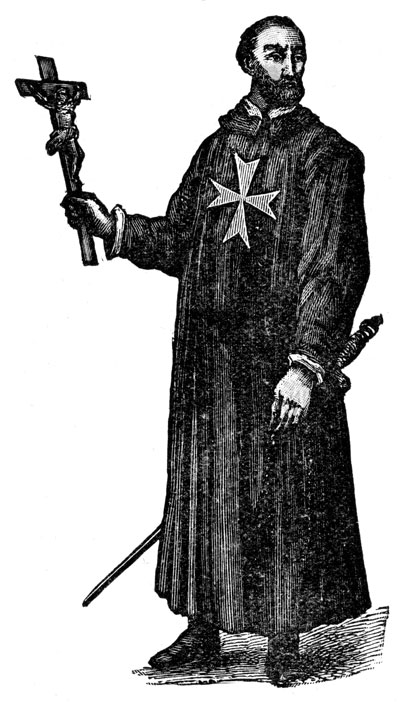
\includegraphics[width=0.25\textwidth]{../images/Cleric.jpg}
\end{center}

\pagebreak

\mysubsection{The Cleric}

The secular world would call them zealots, but Clerics are indeed blessed with power. The Cleric is as much a scholar of their order as they are a knight. Clerics use their divine powers to help allies and repel the forces of darkness.

\bigbreak

The Cleric has the following AV progression:

\bigbreak

\begin{center}
\captionof{table}{CLERIC ATTACK VALUES.}\label{clericav}
\noindent\begin{tabular}{>{\centering\arraybackslash}p{.5\columnwidth -2\tabcolsep}>{\centering\arraybackslash}b{.5\columnwidth -2\tabcolsep}}
\textbf{Cleric Level}&\textbf{Attack Value (AV)}\\
\rowcolor[gray]{0.75}1&11\\
\rowcolor[gray]{0.75}2&11\\
3&12\\
4&12\\
\rowcolor[gray]{0.75}5&12\\
\rowcolor[gray]{0.75}6&13\\
7&13\\
8&14\\
\rowcolor[gray]{0.75}9&14\\
\rowcolor[gray]{0.75}10&14\\
\end{tabular}
\end{center}

\bigbreak

Clerics can ``channel energy" to harm or to heal. The Cleric may heal an ally in sight for d6 health, or harm an enemy in sight for d6 damage, after they \TTN{enemy HD}{WIS}. Clerics may channel energy a number of times equal to their level each day.

\bigbreak

A Cleric may brandish a symbol of authority/sanctity to ``turn undead." If the Cleric \textbf{Threads the Needle} above the HD of an undead and below WIS, then 2d6 present undead of that kind flee from the Cleric for 2d6 rounds. If there are different kinds of undead present, the Cleric must turn them in order of ascending HD. In a single combat encounter, the Cleric may turn undead until one of their attempts fails.

\bigbreak

The Cleric can cast spells from the divine spell list. When a Cleric levels up, they pray to their patron and are blessed with d4+2 spells that the patron chooses.

\bigbreak

When the Cleric casts a spell, they roll a usage die based on their level and the level of the spell as given on \boldref{clericspells}. On a roll of 1 or 2, the usage die is downgraded, or if the die was a d4, the Cleric is out of spells of that level until the following day.

\bigbreak

\begin{center}
\captionof{table}{CLERIC SPELLS PER DAY.}\label{clericspells}
\noindent\begin{tabular}{>{\centering\arraybackslash}b{.15\columnwidth -2\tabcolsep}>{\centering\arraybackslash}p{.094\columnwidth -2\tabcolsep}>{\centering\arraybackslash}p{.094\columnwidth -2\tabcolsep}>{\centering\arraybackslash}p{.094\columnwidth -2\tabcolsep}>{\centering\arraybackslash}p{.094\columnwidth -2\tabcolsep}>{\centering\arraybackslash}p{.094\columnwidth -2\tabcolsep}>{\centering\arraybackslash}p{.094\columnwidth -2\tabcolsep}>{\centering\arraybackslash}p{.094\columnwidth -2\tabcolsep}>{\centering\arraybackslash}p{.094\columnwidth -2\tabcolsep}>{\centering\arraybackslash}p{.094\columnwidth -2\tabcolsep}}
\textbf{Cleric}&\multicolumn{9}{c}{\textbf{Spell usage die for each spell level}}\\
\textbf{Level}&\textbf{1}&\textbf{2}&\textbf{3}&\textbf{4}&\textbf{5}&\textbf{6}&\textbf{7}&\textbf{8}&\textbf{9}\\
\rowcolor[gray]{0.75}1&d4&-&-&-&-&-&-&-&-\\
\rowcolor[gray]{0.75}2&d4&d4&-&-&-&-&-&-&-\\
3&d6&d4&d4&-&-&-&-&-&-\\
4&d6&d6&d4&d4&-&-&-&-&-\\
\rowcolor[gray]{0.75}5&d8&d6&d4&d4&d4&-&-&-&-\\
\rowcolor[gray]{0.75}6&d8&d8&d6&d4&d4&d4&-&-&-\\
7&d10&d8&d6&d6&d4&d4&d4&-&-\\
8&d10&d10&d6&d6&d4&d4&d4&d4&-\\
\rowcolor[gray]{0.75}9&d12&d10&d8&d6&d6&d4&d4&d4&d4\\
\rowcolor[gray]{0.75}10&d12&d12&d8&d8&d6&d6&d4&d4&d4\\
\end{tabular}
\end{center}

\pagebreak

\mysubsection{The Druid}

Druids live in harmony with all of nature, existing in the balance between order and chaos. They hold plants, animals, the sun, and the moon as deities. Through their careful study and protection of the natural world, Druids are blessed with earthly magics and abilities.

\bigbreak

The Druid has the following AV progression:

\bigbreak

\begin{center}
\captionof{table}{DRUID ATTACK VALUES.}\label{druidav}
\noindent\begin{tabular}{>{\centering\arraybackslash}p{.5\columnwidth -2\tabcolsep}>{\centering\arraybackslash}b{.5\columnwidth -2\tabcolsep}}
\textbf{Druid Level}&\textbf{Attack Value (AV)}\\
\rowcolor[gray]{0.75}1&8\\
\rowcolor[gray]{0.75}2&8\\
3&9\\
4&9\\
\rowcolor[gray]{0.75}5&9\\
\rowcolor[gray]{0.75}6&10\\
7&10\\
8&11\\
\rowcolor[gray]{0.75}9&11\\
\rowcolor[gray]{0.75}10&11\\
\end{tabular}
\end{center}

\bigbreak

Druids can sustain themselves off the land. Outside of civilization, a Druid need not consume daily rations, cannot be poisoned, and gains their level in HP when resting, in addition to their die.

\bigbreak

Once per day, the Druid may devote an hour to cast any spell of their level or lower on the nature spell list as an involved and technical ritual. If they are interrupted, the spell fails.

\bigbreak

The Druid can cast spells from the nature spell list. When a Druid levels up, they meditate in nature and are enlightened with d4+2 spells. Druids are social and will share the spells they know with ally Druids, but it takes time to study and perfect the art.

\bigbreak

When the Druid casts a spell, they roll a usage die based on their level and the level of the spell as given on \boldref{druidspells}. On a roll of 1 or 2, the usage die is downgraded, or if the die was a d4, the Druid is out of spells of that level until the following day.

\bigbreak

\begin{center}
\captionof{table}{DRUID SPELLS PER DAY.}\label{druidspells}
\noindent\begin{tabular}{>{\centering\arraybackslash}b{.15\columnwidth -2\tabcolsep}>{\centering\arraybackslash}p{.094\columnwidth -2\tabcolsep}>{\centering\arraybackslash}p{.094\columnwidth -2\tabcolsep}>{\centering\arraybackslash}p{.094\columnwidth -2\tabcolsep}>{\centering\arraybackslash}p{.094\columnwidth -2\tabcolsep}>{\centering\arraybackslash}p{.094\columnwidth -2\tabcolsep}>{\centering\arraybackslash}p{.094\columnwidth -2\tabcolsep}>{\centering\arraybackslash}p{.094\columnwidth -2\tabcolsep}>{\centering\arraybackslash}p{.094\columnwidth -2\tabcolsep}>{\centering\arraybackslash}p{.094\columnwidth -2\tabcolsep}}
\textbf{Druid}&\multicolumn{9}{c}{\textbf{Spell usage die for each spell level}}\\
\textbf{Level}&\textbf{1}&\textbf{2}&\textbf{3}&\textbf{4}&\textbf{5}&\textbf{6}&\textbf{7}&\textbf{8}&\textbf{9}\\
\rowcolor[gray]{0.75}1&d4&-&-&-&-&-&-&-&-\\
\rowcolor[gray]{0.75}2&d4&d4&-&-&-&-&-&-&-\\
3&d6&d4&d4&-&-&-&-&-&-\\
4&d6&d6&d4&d4&-&-&-&-&-\\
\rowcolor[gray]{0.75}5&d8&d6&d4&d4&d4&-&-&-&-\\
\rowcolor[gray]{0.75}6&d8&d8&d6&d4&d4&d4&-&-&-\\
7&d10&d8&d6&d6&d4&d4&d4&-&-\\
8&d10&d10&d6&d6&d4&d4&d4&d4&-\\
\rowcolor[gray]{0.75}9&d12&d10&d8&d6&d6&d4&d4&d4&d4\\
\rowcolor[gray]{0.75}10&d12&d12&d8&d8&d6&d6&d4&d4&d4\\
\end{tabular}
\end{center}

\pagebreak

\begin{center}
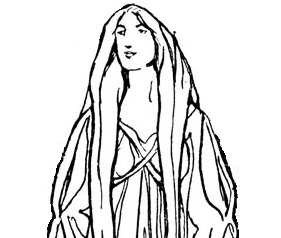
\includegraphics[width=0.25\textwidth]{../images/Druid.jpg}
\end{center}

\mysubsection{The Dwarf}

The Dwarfs are an indulgent coastal people; their love of all that is learned and refined extends from literature, play-writing, painting, and sculpting, to mathematics, philosophy, science, and polemology. Dwarfs are polytheistic, and delight in telling stories about the folly and hubris of their gods.

\bigbreak

The Dwarf has the following AV progression:

\bigbreak

\begin{center}
\captionof{table}{DWARF ATTACK VALUES.}\label{dwarfav}
\noindent\begin{tabular}{>{\centering\arraybackslash}p{.5\columnwidth -2\tabcolsep}>{\centering\arraybackslash}b{.5\columnwidth -2\tabcolsep}}
\textbf{Dwarf Level}&\textbf{Attack Value (AV)}\\
\rowcolor[gray]{0.75}1&11\\
\rowcolor[gray]{0.75}2&11\\
3&12\\
4&12\\
\rowcolor[gray]{0.75}5&13\\
\rowcolor[gray]{0.75}6&13\\
7&14\\
8&14\\
\rowcolor[gray]{0.75}9&15\\
\rowcolor[gray]{0.75}10&15\\
\end{tabular}
\end{center}

\bigbreak

A Dwarf's knowledge of science and medicine allows them to add their level to HP recovered when they bandage injured characters.

\bigbreak

A Dwarf can inspire allies to greatness. At times of rest, the Dwarf may tell their friends a gripping myth or legendary tale. If a listener later finds themselves in similar circumstances to the myth, they may roll a check or save at Advantage. This can be performed once per myth told.

\begin{center}

\includegraphics[width=0.25\textwidth]{../images/Dwarf.jpg}
\end{center}

\pagebreak

\mysubsection{The Elf}

The Elves are a dying race. Their people have been spread to the four winds. The ancient art of Elven study is nearly lost to time. The few desperate Elves that remain have made it their quest to preserve Elven culture, where both magic and might are equally revered. Elves adventure to recover ancient Elven artifacts, to spread the history of the Elves, and to educate the future generations of their spell-sword craft. 

\bigbreak

The Elf has the following AV progression:

\bigbreak

\begin{center}
\captionof{table}{ELF ATTACK VALUES.}\label{elfav}
\noindent\begin{tabular}{>{\centering\arraybackslash}p{.5\columnwidth -2\tabcolsep}>{\centering\arraybackslash}b{.5\columnwidth -2\tabcolsep}}
\textbf{Elf Level}&\textbf{Attack Value (AV)}\\
\rowcolor[gray]{0.75}1&11\\
\rowcolor[gray]{0.75}2&11\\
3&12\\
4&13\\
\rowcolor[gray]{0.75}5&13\\
\rowcolor[gray]{0.75}6&14\\
7&15\\
8&15\\
\rowcolor[gray]{0.75}9&16\\
\rowcolor[gray]{0.75}10&17\\
\end{tabular}
\end{center}

\bigbreak

The years of study and experience that Elves devote to their craft allows them to exert themselves in a desperate ``surge." As many times per day as their level, if an Elf fails a save or check, they may describe how they reassess, readjust, or react to the situation, and reroll the die. An Elf may alternatively spend a surge to add their level to a damage roll.

\bigbreak

An Elf can push themselves beyond the limits of their body and cast additional spells at a cost to their health. If an Elf has run out of spells for the day, they may cast additional spells at the cost of their level in permanent HP lost per spell. 

\bigbreak

The Elf can cast spells from the arcane spell list. An Elf learns one spell each time they level up, but can find more from spellbooks and spellcasters in the world. The number of spells an Elf can cast per day is listed on \boldref{elfspells}.

\bigbreak

\begin{center}
\captionof{table}{ELF SPELLS PER DAY.}\label{elfspells}
\noindent\begin{tabular}{>{\centering\arraybackslash}b{.5\columnwidth -2\tabcolsep}>{\centering\arraybackslash}p{.5\columnwidth -2\tabcolsep}}
\textbf{Elf Level}&\textbf{Spells allotted}\\
\rowcolor[gray]{0.75}1&1\\
\rowcolor[gray]{0.75}2&2\\
3&2\\
4&3\\
\rowcolor[gray]{0.75}5&4\\
\rowcolor[gray]{0.75}6&4\\
7&5\\
8&6\\
\rowcolor[gray]{0.75}9&6\\
\rowcolor[gray]{0.75}10&7\\
\end{tabular}
\end{center}

\pagebreak

\begin{center}

\includegraphics[width=0.2\textwidth]{../images/Elf.png}
\end{center}

\mysubsection{The Fighter}

From heroes of strength, valor, and glory, to fearsome bandit kings and marauders, Fighters are the brawn of a world where might makes right. A skilled Fighter fears no man; their raw power mixed with their delicate finesse makes a Fighter a fearsome killing machine.

\bigbreak

The Fighter has the following AV progression:

\bigbreak

\begin{center}
\captionof{table}{FIGHTER ATTACK VALUES.}\label{fighterav}
\noindent\begin{tabular}{>{\centering\arraybackslash}p{.5\columnwidth -2\tabcolsep}>{\centering\arraybackslash}b{.5\columnwidth -2\tabcolsep}}
\textbf{Fighter Level}&\textbf{Attack Value (AV)}\\
\rowcolor[gray]{0.75}1&11\\
\rowcolor[gray]{0.75}2&12\\
3&12\\
4&13\\
\rowcolor[gray]{0.75}5&14\\
\rowcolor[gray]{0.75}6&14\\
7&15\\
8&16\\
\rowcolor[gray]{0.75}9&16\\
\rowcolor[gray]{0.75}10&17\\
\end{tabular}
\end{center}

\bigbreak

When a Fighter kills an enemy, they may attack another enemy within range. A Fighter may do this as many times as levels they have, so if a Fighter is level 3, they may attack up to four enemies in range, provided the first three attacks are killing blows.

\bigbreak

If a Fighter fails a STR or DEX save and would be dealt damage, they can opt to destroy their shield, if they have one equipped, and ignore the damage.

\begin{center}
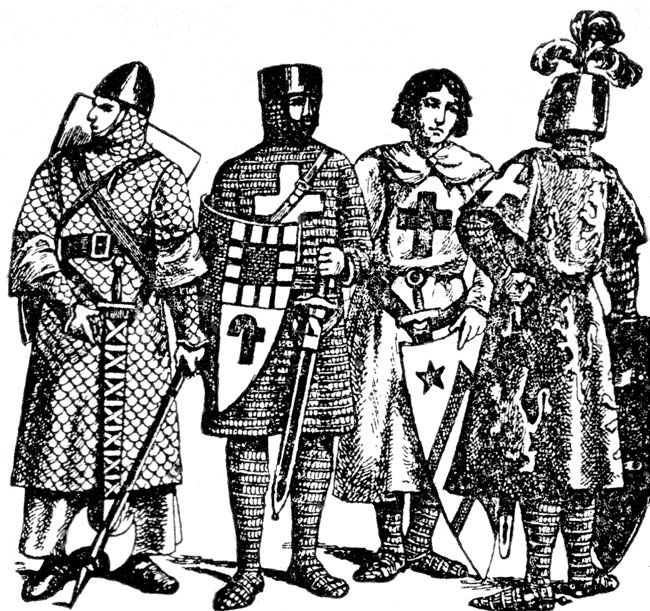
\includegraphics[width=0.25\textwidth]{../images/Fighter.jpg}
\end{center}

\pagebreak

\begin{center}

\includegraphics[width=0.25\textwidth]{../images/Halfling.png}
\end{center}

\mysubsection{The Halfling}

Halflings are cunning tricksters and deviants. They prefer to deal with the riffraff underbelly of society, where they make connections and establish relationships with unsavory characters. A Halfling is not to be trusted, and never fights fair.

\bigbreak

The Halfling has the following AV progression:

\bigbreak

\begin{center}
\captionof{table}{HALFLING ATTACK VALUES.}\label{halflingav}
\noindent\begin{tabular}{>{\centering\arraybackslash}p{.5\columnwidth -2\tabcolsep}>{\centering\arraybackslash}b{.5\columnwidth -2\tabcolsep}}
\textbf{Halfling Level}&\textbf{Attack Value (AV)}\\
\rowcolor[gray]{0.75}1&12\\
\rowcolor[gray]{0.75}2&12\\
3&12\\
4&12\\
\rowcolor[gray]{0.75}5&13\\
\rowcolor[gray]{0.75}6&13\\
7&13\\
8&13\\
\rowcolor[gray]{0.75}9&14\\
\rowcolor[gray]{0.75}10&14\\
\end{tabular}
\end{center}

\bigbreak

If a Halfling successfully attacks an enemy from an advantageous position, they may do additional damage equal to their level.

\bigbreak

Each time the Halfling levels up, they gain 3d6$\times$their level gold worth of favors to collect. The favors can be used for anything agreed upon by player and Referee.

\begin{center}
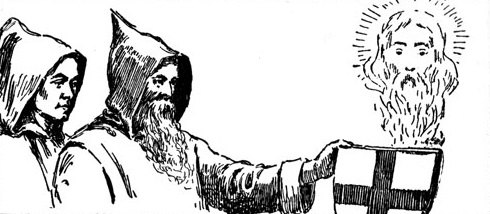
\includegraphics[width=0.4\textwidth]{../images/Magic-User.jpg}
\end{center}

\pagebreak

\mysubsection{The Magic-User}

Whether a born natural or a devoted student of the arts, a Magic-User has unearthly abilities at their very fingers. Magic-Users bend reality to their whims, and thus many obstacles become trivial to a creative Magic-User. Magic-Users think outside the box, using their spells and powers to circumvent problems and avoid confrontation.

\bigbreak

The Magic-User has the following AV progression:

\bigbreak

\begin{center}
\captionof{table}{MAGIC-USER ATTACK VALUES.}\label{magicuserav}
\noindent\begin{tabular}{>{\centering\arraybackslash}p{.5\columnwidth -2\tabcolsep}>{\centering\arraybackslash}b{.5\columnwidth -2\tabcolsep}}
\textbf{Magic-User Level}&\textbf{Attack Value (AV)}\\
\rowcolor[gray]{0.75}1&8\\
\rowcolor[gray]{0.75}2&8\\
3&8\\
4&9\\
\rowcolor[gray]{0.75}5&9\\
\rowcolor[gray]{0.75}6&9\\
7&10\\
8&10\\
\rowcolor[gray]{0.75}9&10\\
\rowcolor[gray]{0.75}10&11\\
\end{tabular}
\end{center}

\bigbreak

A Magic-User's deep understanding of the arcane arts allows them to unlock extreme magical power through ``metamagic." As many times per day as their level, a Magic-User can do the following: ignore the result of a spell's usage die roll, treat their level as double for the purposes of spell effects, reverse the effects of a spell, cast a spell discreetly, cast a spell without requirements, or cast two spells in one action.

\bigbreak

Once per day, the Magic-User may devote an hour to cast any spell on the arcane spell list as an involved and technical ritual. If they are interrupted, the spell fails.

\bigbreak

The Magic-User can cast spells from the arcane spell list. A Magic-User learns one spell each time they level up, but can find more from spellbooks and spellcasters in the world. When the Magic-User casts a spell, they roll a usage die based on their level as given on \boldref{magicuserspells}. On a roll of 1 or 2, the usage die is downgraded, or if the die was a d4 with no subsequent dice, the Magic-User is out of spells until the following day. For levels 7 and up, the usage die ``prestiges" and gains subsequent dice; for example, the chain for level 8 is d6>d4>d20>d12>d10>d8>d6>d4.

\bigbreak

\begin{center}
\captionof{table}{MAGIC-USER SPELLS PER DAY.}\label{magicuserspells}
\noindent\begin{tabular}{>{\centering\arraybackslash}b{.5\columnwidth -2\tabcolsep}>{\centering\arraybackslash}p{.5\columnwidth -2\tabcolsep}}
\textbf{Magic-User Level}&\textbf{Spell usage die}\\
\rowcolor[gray]{0.75}1&d4\\
\rowcolor[gray]{0.75}2&d6\\
3&d8\\
4&d10\\
\rowcolor[gray]{0.75}5&d12\\
\rowcolor[gray]{0.75}6&d20\\
7&d4, then d20\\
8&d6, then d20\\
\rowcolor[gray]{0.75}9&d8, then d20\\
\rowcolor[gray]{0.75}10&d10, then d20\\
\end{tabular}
\end{center}

\pagebreak

\mysubsection{The Paladin}

A noble, righteous, and holy knight, the Paladin is the embodiment of the virtues they hold dear. In turn, the Paladin is granted power to heal and protect the innocent.

\bigbreak

The Paladin has the following AV progression:

\bigbreak

\begin{center}
\captionof{table}{PALADIN ATTACK VALUES.}\label{paladinav}
\noindent\begin{tabular}{>{\centering\arraybackslash}p{.5\columnwidth -2\tabcolsep}>{\centering\arraybackslash}b{.5\columnwidth -2\tabcolsep}}
\textbf{Paladin Level}&\textbf{Attack Value (AV)}\\
\rowcolor[gray]{0.75}1&11\\
\rowcolor[gray]{0.75}2&11\\
3&12\\
4&12\\
\rowcolor[gray]{0.75}5&13\\
\rowcolor[gray]{0.75}6&13\\
7&14\\
8&14\\
\rowcolor[gray]{0.75}9&15\\
\rowcolor[gray]{0.75}10&15\\
\end{tabular}
\end{center}

\bigbreak

A Paladin can ``lay on hands" to cure wounds. Touching heals d6 damage. Paladins may lay on hands a number of times equal to their level each day.

\bigbreak

During combat, a Paladin may selflessly use their body to shield allies by \textbf{Threading the Needle} above the HD of enemies and below CHA. Until the Paladin's next turn, this maneuver forces all attacks that would target an adjacent ally to target the Paladin instead.

\bigbreak

Starting at level 4, the Paladin can learn and cast spells from the divine spell list. When a Paladin levels up, they pray to their patron and are blessed with 2 spells that the patron chooses.

\bigbreak

The number of spells of each level a Paladin can cast per day is listed on \boldref{paladinspells}.

\bigbreak

\begin{center}
\captionof{table}{PALADIN SPELLS PER DAY.}\label{paladinspells}
\noindent\begin{tabular}{>{\centering\arraybackslash}b{.2\columnwidth -2\tabcolsep}>{\centering\arraybackslash}p{.2\columnwidth -2\tabcolsep}>{\centering\arraybackslash}p{.2\columnwidth -2\tabcolsep}>{\centering\arraybackslash}p{.2\columnwidth -2\tabcolsep}>{\centering\arraybackslash}p{.2\columnwidth -2\tabcolsep}}
\textbf{Paladin}&\multicolumn{4}{c}{\textbf{Spells allotted for each spell level}}\\
\textbf{Level}&\textbf{1}&\textbf{2}&\textbf{3}&\textbf{4}\\
\rowcolor[gray]{0.75}4&1&-&-&-\\
5&2&-&-&-\\
\rowcolor[gray]{0.75}6&2&1&-&-\\
7&2&2&-&-\\
\rowcolor[gray]{0.75}8&2&2&1&-\\
9&3&2&2&-\\
\rowcolor[gray]{0.75}10&3&2&2&1\\
\end{tabular}
\end{center}

\begin{center}
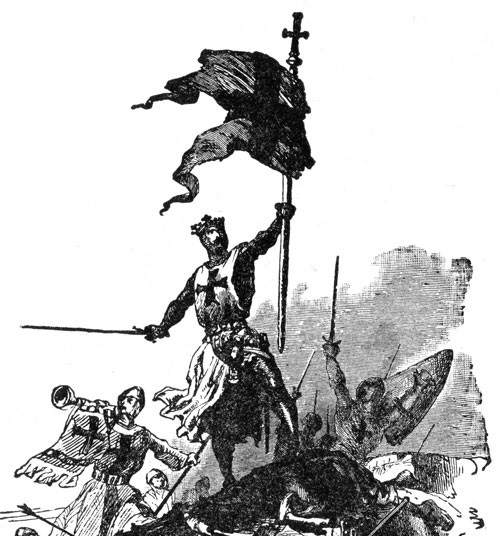
\includegraphics[width=0.2\textwidth]{../images/Paladin.jpg}
\end{center}

\pagebreak

\mysubsection{The Ranger}

Adept at tracking, scouting, infiltration, and hunting, the Ranger has a uniquely specialized set of survival skills. Their abilities make them equally capable combatants and skilled naturalists.

\bigbreak

The Ranger has the following AV progression:

\bigbreak

\begin{center}
\captionof{table}{RANGER ATTACK VALUES.}\label{rangerav}
\noindent\begin{tabular}{>{\centering\arraybackslash}p{.5\columnwidth -2\tabcolsep}>{\centering\arraybackslash}b{.5\columnwidth -2\tabcolsep}}
\textbf{Ranger Level}&\textbf{Attack Value (AV)}\\
\rowcolor[gray]{0.75}1&11\\
\rowcolor[gray]{0.75}2&11\\
3&12\\
4&12\\
\rowcolor[gray]{0.75}5&13\\
\rowcolor[gray]{0.75}6&13\\
7&14\\
8&14\\
\rowcolor[gray]{0.75}9&15\\
\rowcolor[gray]{0.75}10&15\\
\end{tabular}
\end{center}

\bigbreak

Once during each combat, a Ranger may declare an enemy their quarry. Singling out an enemy, a Ranger marks them for death and hones their attacks amidst the chaos of battle. Against this enemy, the Ranger adds their level to all damage rolls.

\bigbreak

A Ranger can travel effortlessly where others would struggle. Choose a favored terrain; examples include desert, hills, forests, jungle, mountains, plains, swamps, tundra, and so on. When in their favored terrain, the Ranger can travel quickly, track parties effortlessly, travel without leaving a trace, and avoid encountering man. This ability extends to the Ranger's companions, provided they follow the Ranger's guidance.

\bigbreak

Starting at level 4, the Ranger can learn and cast spells from the nature spell list. When a Ranger levels up, they meditate in nature and are enlightened with 2 spells. 

\bigbreak

The number of spells of each level a Ranger can cast per day is listed on \boldref{rangerspells}.

\bigbreak

\begin{center}
\captionof{table}{RANGER SPELLS PER DAY.}\label{rangerspells}
\noindent\begin{tabular}{>{\centering\arraybackslash}b{.2\columnwidth -2\tabcolsep}>{\centering\arraybackslash}p{.2\columnwidth -2\tabcolsep}>{\centering\arraybackslash}p{.2\columnwidth -2\tabcolsep}>{\centering\arraybackslash}p{.2\columnwidth -2\tabcolsep}>{\centering\arraybackslash}p{.2\columnwidth -2\tabcolsep}}
\textbf{Ranger}&\multicolumn{4}{c}{\textbf{Spells allotted for each spell level}}\\
\textbf{Level}&\textbf{1}&\textbf{2}&\textbf{3}&\textbf{4}\\
\rowcolor[gray]{0.75}4&1&-&-&-\\
5&2&-&-&-\\
\rowcolor[gray]{0.75}6&2&1&-&-\\
7&2&2&-&-\\
\rowcolor[gray]{0.75}8&2&2&1&-\\
9&3&2&2&-\\
\rowcolor[gray]{0.75}10&3&2&2&1\\
\end{tabular}
\end{center}

\pagebreak

\begin{center}
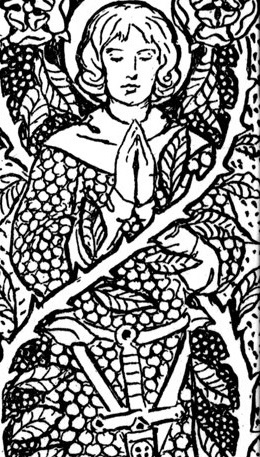
\includegraphics[width=0.25\textwidth]{../images/Ranger.jpg}
\end{center}

\mysubsection{The Warlock}

To the unlearned peasant, Warlocks must seem like gods. They have the ability to warp the essential fabric of reality; physics and nature bend to their very will. But there is something decidedly unnatural about having such power. It is said that Warlocks are corrupted by their power, but perhaps these are rumors spread by the untalented mundane world. There are murmurs that Warlocks must make pacts with eldritch nightmares to earn their arcane abilities. Such gossip is dismissed as fancy by Warlocks, but of course it would be.

\bigbreak

The Warlock has the following AV progression:

\bigbreak

\begin{center}
\captionof{table}{WARLOCK ATTACK VALUES.}\label{warlockav}
\noindent\begin{tabular}{>{\centering\arraybackslash}p{.5\columnwidth -2\tabcolsep}>{\centering\arraybackslash}b{.5\columnwidth -2\tabcolsep}}
\textbf{Warlock Level}&\textbf{Attack Value (AV)}\\
\rowcolor[gray]{0.75}1&8\\
\rowcolor[gray]{0.75}2&8\\
3&8\\
4&9\\
\rowcolor[gray]{0.75}5&9\\
\rowcolor[gray]{0.75}6&9\\
7&10\\
8&10\\
\rowcolor[gray]{0.75}9&10\\
\rowcolor[gray]{0.75}10&11\\
\end{tabular}
\end{center}

\bigbreak

The Warlock does not learn spells of their own accord. They are given (or blessed, or cursed) spells by supernatural eldritch horrors with no concern for the machinations of man. Each time the Warlock gains a level, in the back of their dreams whispers an ancient being with a snarling cadence and a melodious wail. It has all the answers the Warlock seeks, and more. For a ``mundane" task, something truly ``trivial," it will grant the Warlock the powers they so desperately deserve. By fulfilling the task, the Warlock gains d5-1 spells from the Necronomicon spell list.

\bigbreak

When the Warlock casts a spell, they roll a usage die based on their level as given on \boldref{warlockspells}. On a roll of 1 or 2, the usage die is downgraded, or if the die was a d4, the Warlock is out of spells until the following day. Note that a Warlock's usage die chain differs from all other usage die chains: d20>d16>d14>d12>d10>d8>d7>d6>d5>d4.

\bigbreak

\begin{center}
\captionof{table}{WARLOCK SPELLS PER DAY.}\label{warlockspells}
\noindent\begin{tabular}{>{\centering\arraybackslash}b{.5\columnwidth -2\tabcolsep}>{\centering\arraybackslash}p{.5\columnwidth -2\tabcolsep}}
\textbf{Warlock Level}&\textbf{Spell usage die}\\
\rowcolor[gray]{0.75}1&d4\\
\rowcolor[gray]{0.75}2&d5\\
3&d6\\
4&d7\\
\rowcolor[gray]{0.75}5&d8\\
\rowcolor[gray]{0.75}6&d10\\
7&d12\\
8&d14\\
\rowcolor[gray]{0.75}9&d16\\
\rowcolor[gray]{0.75}10&d20\\
\end{tabular}
\end{center}

\bigbreak

The Warlock is not left unscathed from their encounters with eldritch beings. Each time a Warlock levels up and completes their favors to learn new spells, they also gain a Corruption point. Additionally, Warlocks that stretch themselves to breaking and cast more spells in one day than what their body and mind can handle will also take on Corruption points; when a Warlock reaches their daily limit, they may cast additional spells at the cost of one Corruption point and one Corruption check per spell. Corruption can also be earned through horrible and unspeakable deeds not dared written here. 

\bigbreak

In times of great stress and anguish, a Warlock may be pushed to their limit. The Referee should ask the Warlock to roll a d20 in a Corruption check. If they roll \emph{above} their Corruption score, they are safe for yet another day (\emph{but at what cost?}). If, however, the roll ties or is lower than their Corruption score, the Warlock is fully seized by the madness inherent in their terrible art. Such Warlocks will not adventure with their companions any longer. They may be dragged to hell by the demons they once confided in; they may be driven mad and flee to start a cult in a mountain of power; they may attack the men and women they once called their friends before they turn on themselves. It is always a terrible moment.

\begin{center}

\includegraphics[width=0.35\textwidth]{../images/Warlock.png}
\end{center}

\pagebreak

\mysection{MAGIC}

Magic is divided into four distinct flavors: arcane, divine, natural, and necrotic. Choice of class determines which spells a character is able to cast. 

\bigbreak

Elves and Magic-Users cast spells from the arcane spell list. These spells have no inherent level; a caster can cast any spell that they know or have access to, and the effects of that spell are scaled based on the level of the caster. Arcane spells are utility spells, able to solve problems and influence circumstances.

\bigbreak

Clerics and Paladins cast spells from the divine spell list. These spells are ranked by level; higher level spells are more powerful and can only be cast by higher level characters. Divine spells deal in life and death, good and evil, and the forces of the gods.

\bigbreak

Druids and Rangers cast spells from the nature spell list. These spells are ranked by level; higher level spells are more powerful and can only be cast by higher level characters. Nature spells influence the natural world, gaining information from and lording power over plants and animals.

\bigbreak

Warlocks cast spells from the Necronomicon. These spells have no inherent level; a caster can cast any spell that they know, and the effects of that spell are scaled based on the level of the caster. Necrotic spells inflict pain and suffering and force enemies to submit to commands and influences against their will.

\mysubsection{Arcane Spells}

Below is a list of some of the arcane spells in existence. In the following list, ``$\ell$" is a number equal to the caster’s level. Unless otherwise noted, all spells with ongoing effects last up to $\ell\times$10 minutes, and have a range of up to 40 feet. If the target attempts to resist the spell, the caster must \TTN{target HD}{their spellcasting stat (INT for Elves and Magic-Users)}. If they fail, the effects of the spell are reduced or negated.

\textbf{\ref*{arc:num} Arcane Spells}
\begin{enumerate}[nosep]
\item \textbf{Adhere}: Your touched target exudes a thick, white, pasty glue. It becomes extremely sticky.
\item \textbf{Aeromancer}: Invoke and control wind up to the intensity of a light breeze.
\item \textbf{Aethersight}: Magic auras glow in the color of song. You can discern when objects have been magically affected or when casters are being discreet.
\item \textbf{Allure}: Creatures within sight are compelled to approach you, but do not change their disposition towards you.
\item \textbf{Animate}: You control an inanimate object.
\item \textbf{Animate Shadow}: Your shadow disconnects from you but remains under your control.
\item \textbf{Arcane Eye}: Your eyeball detaches and you can see through it as it flies at your command.
\item \textbf{Astral Prison}: A surge freezes the target in time and space within an invulnerable crystal shell.
\item \textbf{Astral Shield}: An incorporeal barrier forms in the air.
\item \textbf{Astral Weapon}: A heroic weapon of legend, your choice, appears.
\item \textbf{Attract}: $\ell$+1 objects are magnetically attracted to one another if they come within 10 feet.
\item \textbf{Auditory Illusion}: You create illusory noises that appear to come from a direction of your choice.
\item \textbf{Babble}: The target must clearly say everything you think but is otherwise mute.
\item \textbf{Banish Cube}: You may destroy 3 foot wide cubes of soil once a round.
\item \textbf{Beacon}: The target emits a black psychic pulse that draws the curiosity of all monsters within 1 mile.
\item \textbf{Befuddle}: $\ell$ targets cannot form memories, tell creatures apart, or otherwise act intelligently.
\item \textbf{Bend Fate}: Roll $\ell+1$ d20s. Each time you roll a d20, choose one of the rolled results until they are gone.
\item \textbf{Blood::Water::Wine}: Transform one of blood, water, or wine into another.
\item \textbf{Body Swap}: You temporarily switch bodies with the target. If one body dies, so does the other.
\item \textbf{Cacophony}: An overwhelming sound fills the area.
\item \textbf{Catherine}: A human named Catherine appears until the spell ends. She will obey polite, safe requests.
\item \textbf{Charm}: $\ell$ targets treat you as a friend.
\item \textbf{Chatter}: $\ell$ targets appear to discuss a topic of your choosing when they speak. Among each other, they hear the true speech.
\item \textbf{Clean}: A target is magically cleaned.
\item \textbf{Coal Stone}: Turn a gem into a source of heat/fire.
\item \textbf{Combine Powers}: Concentrate on this spell to add your caster level to an ally caster.
\item \textbf{Command}: The target obeys a three word command that does not harm it.
\item \textbf{Comprehend}: You become fluent in all languages.
\item \textbf{Compress Space}: Make an area shorter or narrower.
\item \textbf{Control Weather}: You can alter the type of weather at will, but after, the energy can cause natural disasters.
\item \textbf{Darkness}: A shroud blocks all vision in an area.
\item \textbf{Darkvision}: You can see in total darkness.
\item \textbf{Deafen}: All nearby creatures are deafened.
\item \textbf{Decrease Gravity}: The gravity in the area halves.
\item \textbf{D\'ej\`a Vu}: For $\ell$ rounds, a touched target experiences everything twice.
\item \textbf{Delay Danger}: Delay the effects of an attack, spell, trap, etc., which targets you for up to $\ell$ rounds. The effects can be activated at any time during the duration but they must occur once time is up.
\item \textbf{Delay Potion}: Delay the effects of a consumed liquid for up to $\ell$ hours. The effects can be activated at any time during the duration but they must occur once time is up.
\item \textbf{Disassemble}: Any of your body parts may be removed and attached at will. You can control them.
\item \textbf{Disguise}: You disguise $\ell$ targets.
\item \textbf{Displace}: Shift target's apparent place by $\ell\times$10 feet.
\item \textbf{Dizzy Drunkard}: Unbalance $\ell$ targets.
\item \textbf{Earthfast}: Reinforce a rock formation or wood/stone structure.
\item \textbf{Earthquake}: The ground shakes for $\ell$ rounds.
\item \textbf{Elasticity}: Your body can stretch up to $\ell\times$10 feet.
\item \textbf{Elemental Wall}: An $\ell\times$40 foot long wall of ice, fire, or other element blasts from the ground.
\item \textbf{Eraser}: Erase writing. Magical writing resists this spell and requires a roll.
\item \textbf{Faegold}: Create a coin that vanishes in 10 minutes.
\item \textbf{Feast}: A huge table appears with delicious food.
\item \textbf{Feather}: $\ell$ falling/flying/propelled items become as light as feathers.
\item \textbf{Filch}: $\ell$ visible items teleport to your hands.
\item \textbf{Flatten}: You become two dimensional.
\item \textbf{Flavor}: The target is more appetizing.
\item \textbf{Fog Cloud}: Dense black fog spreads out from you.
\item \textbf{Frenzy}: $\ell$ creatures erupt in senseless violence.
\item \textbf{Gate Gossip}: A door tells you either the name and nature of the last three creatures, or the number of creatures that day, to pass through it.
\item \textbf{Glass Form}: A touched surface becomes see-through up to $\ell$ feet. Lead and silver are immune.
\item \textbf{Gravity Shift}: You can change the direction of gravity for yourself once per round.
\item \textbf{Grease}: Cast forth a spurt of grease, which can cover $\ell\times$10 square feet.
\item \textbf{Greed}: $\ell$ creatures develop an overwhelming urge to possess a visible item of your choice.
\item \textbf{Grow}: Double the size of a touched target.
\item \textbf{Haste}: $\ell$ touched targets move three times as fast.
\item \textbf{Hear Whispers}: A touched target hears the faintest of sounds.
\item \textbf{Hold Closed}: A closed door can't be opened by anyone but the caster (but it can still be destroyed).
\item \textbf{Hold Open}: An open door can't be closed by anyone but the caster.
\item \textbf{Hover}: An object hovers 2 feet off the ground. It can hold $\ell$ men.
\item \textbf{Hypnotize}: The target enters a dreamy trance and will truthfully answer $\ell$ questions. 
\item \textbf{Ice}: An $\ell\times$10 foot radius of ice spreads from a point.
\item \textbf{Increase Gravity}: The gravity in the area doubles.
\item \textbf{Invisible Tether}: Two objects must remain less than 10 feet apart.
\item \textbf{Knock}: $\ell$ nearby locks, clasps, or buckles open.
\item \textbf{Leap}: A touched target can jump $\ell\times$10 feet in the air.
\item \textbf{Life Line}: Link two targets; one need not eat nor breathe, and the other must eat and breathe for both.
\item \textbf{Light}: A floating light moves as you command.
\item \textbf{Liquid Air}: The air becomes thick enough to swim in.
\item \textbf{Magic Dampener}: Nearby magic has effects halved.
\item \textbf{Magic Mouth}: Enchant an object to deliver a message once a condition is triggered.
\item \textbf{Manipulate Clockwork}: You affect a minor change in a small mechanical item.
\item \textbf{Manse}: A furnished cottage appears for $\ell\times$12 hours.
\item \textbf{Marble Madness}: Your pockets are always full of marbles.
\item \textbf{Masquerade}: $\ell$ creatures turn identical to a target.
\item \textbf{Metal Melt}: A touched metal becomes cool liquid and rehardens in 1 round.
\item \textbf{Miniaturize}: $\ell$ touched creatures are mouse-sized.
\item \textbf{Mirror Image}: $\ell$ copies of yourself appear.
\item \textbf{Mirrorwalk}: A mirror becomes a gate to another mirror that you have looked into today.
\item \textbf{Multiarm}: You gain $\ell$ extra arms.
\item \textbf{Multihead}: You gain $\ell$ extra heads.
\item \textbf{Multileg}: You gain $\ell$ extra legs.
\item \textbf{Multitask}: Split your mind in two and perform twice as many actions for $\ell$ rounds. When this spell ends, roll a CON save or collapse in exhaustion.
\item \textbf{Night Orb}: A $\ell\times$40 foot radius ball of night appears.
\item \textbf{Objectify}: You become an inanimate object.
\item \textbf{Ooze Form}: You melt into a living jelly.
\item \textbf{Pacify}: $\ell$ targets have a sudden aversion to violence.
\item \textbf{Phantom Coach}: A coach arrives, slightly translucent in direct light, emitting billowing wisps of night. It moves unnaturally fast over any terrain, even water.
\item \textbf{Phobia}: $\ell$ targets are terrified of an object you choose.
\item \textbf{Photo}: Instantly transcribe what you see to paper.
\item \textbf{Pit}: A pit 10 feet wide and $\ell\times$5 feet deep appears.
\item \textbf{Presence}: The target feels as though they are being watched.
\item \textbf{Primeval Surge}: An object is grown to the size of an elephant. If it is an animal, it is enraged.
\item \textbf{Psychometry}: Discern the answers to $\ell$ yes/no questions about a touched object.
\item \textbf{Pull}: An object is pulled with the strength of $\ell$ men for 1 round.
\item \textbf{Push}: An object is pushed with the strength of $\ell$ men for 1 round.
\item \textbf{Quench}: Extinguish a small controlled flame, like a torch or campfire.
\item \textbf{Raise Spirit}: For a favor, a touched corpse's spirit appears and answers $\ell$ questions.
\item \textbf{Read Mind}: You hear thoughts of creatures nearby.
\item \textbf{Repel}: $\ell$+1 objects are magnetically repelled from each other if they come within 10 feet.
\item \textbf{Root}: Touched target cannot be moved against their will.
\item \textbf{Scribe}: Copy 1 page of text, or transcribe what is said for $\ell$ minutes.
\item \textbf{Scry}: You see the POV of a creature touched today.
\item \textbf{Sculpt Elements}: Inanimate material behaves like wet clay in your hands.
\item \textbf{Share Senses}: You and a touched target freely exchange sensory information.
\item \textbf{Shrink}: Halve the size of a touched target.
\item \textbf{Shroud}: $\ell$ targets are invisible until they move.
\item \textbf{Shuffle}: $\ell$ targets randomly switch places.
\item \textbf{Sigil of Channeling}: Inscribe a sigil on an object or person to be able to cast spells as if you are at the location of the sigil. The sigil remains for $\ell$ hours.
\item \textbf{Sixth Sense}: You cannot be surprised.
\item \textbf{Skunk}: A bad smell fills the area.
\item \textbf{Sleep}: $\ell$ creatures fall into a light sleep.
\item \textbf{Sleepwalk}: You can act during a full night's rest. You cannot use this spell to gain the benefits of rest more than once per day.
\item \textbf{Slow Spell}: In a chosen area, spells occur 1 round after they are cast.
\item \textbf{Smoke Form}: Your body becomes living smoke.
\item \textbf{Snail Knight}: A time after casting, a knight astride a giant snail rides into view. He answers most questions related to quests, and may aid you if you are worthy.
\item \textbf{Sniff}: A touched target smells the faintest traces of scents.
\item \textbf{Soil}: A target is magically dirtied.
\item \textbf{Sort}: Inanimate items sort themselves as you specify.
\item \textbf{Sour}: The target is more unappetizing.
\item \textbf{Spatial Distortion}: A nearby object shrinks to the size of an apple.
\item \textbf{Spectacle}: A clearly unreal but impressive illusion appears under your control, with motion and sound.
\item \textbf{Spellseize}: Remove a spell from a caster's mind and store it to cast later. After casting, the spell is gone.
\item \textbf{Spider Climb}: A target climbs surfaces like a spider.
\item \textbf{Stone::Flesh}: Transform stone into flesh, or vice versa.
\item \textbf{Stretch Space}: Make an area longer or wider.
\item \textbf{Summon Cube}: You may create 3 foot wide cubes of soil once a round.
\item \textbf{Summon Idol}: A carved idol rises from the ground.
\item \textbf{Swarm}: You become a swarm of crows, rats, or piranha.
\item \textbf{Taste}: A touched target tastes the faintest of sapors.
\item \textbf{Telekinesis}: You may mentally move $\ell$ items.
\item \textbf{Telepathy}: $\ell+1$ targets hear each other's thoughts.
\item \textbf{Teleport}: An object teleports up to $\ell\times$40 feet.
\item \textbf{Thaumaturgic Anchor}: The target becomes the target of all spells cast near it, and all casters must roll under their spellcasting stat to target anything else.
\item \textbf{Time Jump}: The target hurls itself up to $\ell\times$10 minutes into the future.
\item \textbf{Time Pocket}: You dislocate in time for up to $\ell$ minutes. You can see and be seen by creatures in normal time, but as if in a fog. You ignore all effects and objects other than those that originate with you. Likewise, you cannot affect normal time.
\item \textbf{Time Rewind}: Time in a chosen area flows backwards.
\item \textbf{Time Rush}: Time in a chosen area becomes 10 times faster.
\item \textbf{Time Share}: You give the target your time. It can act on your turn as if it were its own. You are petrified until the end of your turn.
\item \textbf{Time Slow}: Time in a chosen area becomes 10 times slower.
\item \textbf{Trade Luck}: You gain Advantage and a target gains Disadvantage on all d20 rolls.
\item \textbf{Transcribe Sigil}: Touch a magical sigil, glyph, or symbol to pick it up. Make a save or it activates, targeting you. You must set it down before the spell ends.
\item \textbf{Transfer Heat}: Transfer heat between two targets.
\item \textbf{Tremorsense}: Your sense of touch heightens.
\item \textbf{True Sight}: You see through all illusions.
\item \textbf{Upwell}: A spring of seawater appears.
\item \textbf{Ventriloquism}: Project your voice to a different place.
\item \textbf{Vision}:  You control what a target sees.
\item \textbf{Visual Illusion}: A silent immobile illusion appears.
\item \textbf{Ward}: A silver ring of radius 40 feet appears. Choose one thing that cannot cross it: the living, the dead, projectiles, or metal.
\item \textbf{Web}: Your hands can shoot thick webbing.
\item \textbf{Wizard Lock}: A close-able thing is magically sealed.
\item \textbf{Wizard Mark}: You can leave marks visible only to casters that can be seen at any distance and through solid objects.
\item \textbf{Wristpocket}: A held object can be hidden in an extradimensional space and retrieved at will.
\item \textbf{X-Ray Vision}: You gain X-ray vision.
\label{arc:num}
\end{enumerate}

\mysubsection{Divine Spells}

Below is a list of some of the divine spells in existence. Unless otherwise noted, all spells with ongoing effects last up to spell level$\times$10 minutes, and have a range of up to 40 feet. If the target attempts to resist the spell, the caster must \TTN{target HD}{their spellcasting stat (WIS for Clerics, CHA for Paladins)}. If they fail, the effects of the spell are reduced or negated.

\textbf{Level 1 Divine Spells}
\begin{enumerate}[nosep]
\item \textbf{Alacrity}: For the rest of the day, your touched target has Advantage on initiative rolls.
\item \textbf{Combine Powers}: Concentrate on this spell to add your caster level to an ally caster.
\item \textbf{Cure Light Wounds}: Target heals d8 HP.
\item \textbf{Detect Undead}: Nearby undead glow.
\item \textbf{Inflict Light Wounds}: Target loses d8 HP.
\item \textbf{Light}: A floating light moves as you command.
\item \textbf{Message}: Send a discreet message up to 1 mile.
\item \textbf{Protection From Evil}: Gain Advantage on all rolls against Evil.
\item \textbf{Purify Food/Water}: Remove disease from food/water.
\item \textbf{Resist Cold}: The target is immune to mundane cold and gains Advantage against magical cold.
\item \textbf{Rousing Cry}: Allies gain Advantage on morale rolls.
\item \textbf{Sanctify Corpse}: Prevent corpse from turning undead.
\item \textbf{Sanctuary}: As long as you remain pacifist, roll with Advantage on saves.
\end{enumerate}

\textbf{Level 2 Divine Spells}
\begin{enumerate}[nosep]
\item \textbf{Augury}: Determine whether a future action will bring weal or woe.
\item \textbf{Bless}: Allies gain +1 to stats and AV when attacking and saving for 1 hour.
\item \textbf{Command}: The target obeys a three word command that does not harm it.
\item \textbf{Detect Evil}: Nearby Evil glows.
\item \textbf{Hold Person}: Paralyze d4 targets. Roll each round to maintain the hold; the effect lasts until the roll fails.
\item \textbf{Life Pact}: Link two targets; if one falls below 0 HP, the other loses enough HP to bring the first back to 0 HP.
\item \textbf{Magic Appraisal}: Touch an object. You learn one: who last possessed it, who created it, how to fix it, what it's used for, where to use it, or where to sell it.
\item \textbf{Martyr's Bargain}: Delay all damage in a round to take maximum damage in the following round.
\item \textbf{Resist Fire}: The target is immune to mundane heat and gains Advantage against magical heat.
\item \textbf{Silence}: No sound can pass through a specified area.
\item \textbf{Speak With Animals}: Speak to/understand animals.
\end{enumerate}

\textbf{Level 3 Divine Spells}
\begin{enumerate}[nosep]
\item \textbf{Cause Disease}: Inflict a target with a disease.
\item \textbf{Cure Disease}: Cure a target of a disease.
\item \textbf{Daylight}: An area is illuminated with sunlight.
\item \textbf{Greater Augury}: Determine whether the next hour will be safe, perilous, or bring great danger.
\item \textbf{Locate}: Discern the direction of a known object.
\item \textbf{Prayer}: Allies gain Advantage when attacking and saving for 1 combat.
\item \textbf{Raise Spirit}: For a favor, a touched corpse's spirit appears and answers 3 questions.
\item \textbf{Remove Curse}: Remove a curse from a target.
\item \textbf{Truthsense}: You know when an observed target is dishonest.
\item \textbf{Ward}: A silver ring of radius 40 feet appears. Choose one thing that cannot cross it: the living, the dead, projectiles, or metal.
\end{enumerate}

\textbf{Level 4 Divine Spells}
\begin{enumerate}[nosep]
\item \textbf{Clear Mind}: Target no longer suffers from mental affliction, like madness, mind control, drunkenness, etc. 
\item \textbf{Consecrate}: In an area, undead have 1 less HD.
\item \textbf{Cure Serious Wounds}: Target heals 2d8+1 HP.
\item \textbf{Feast}: A huge table appears with delicious food.
\item \textbf{Superior Augury}: The next hour is actually a dream; after 1 hour is up, the timeline is reset back to the moment of casting, and you retain your knowledge of one possible sequence of events. At the end of this spell, you can choose not to reset; this was the true timeline.
\item \textbf{Heart Sight}: Know the intentions and character of a touched target.
\item \textbf{Hold Undead}: Nearby undead are paralyzed for 4 rounds.
\item \textbf{Inflict Serious Wounds}: Target loses 2d8+1 HP.
\item \textbf{Neutralize Poison}: Remove or immunize vs. poison.
\item \textbf{Prevent Lies}: Creatures within range that attempt to tell a direct lie cannot speak.
\item \textbf{Sticks::Snakes}: Transform sticks into snakes, or vice versa.
\end{enumerate}

\textbf{Level 5 Divine Spells}
\begin{enumerate}[nosep]
\item \textbf{Checkpoint}: If the target dies today, their body and gear disintegrate and they reappear in the same condition as when the spell was cast (including stats, gear, memory, etc.).
\item \textbf{Commune}: Directly ask a deity 3 questions.
\item \textbf{Cure Critical Wounds}: Target heals 3d8+2 HP.
\item \textbf{Dispel Evil}: Remove and negate an Evil spell.
\item \textbf{Inflict Critical Wounds}: Target loses 3d8+2 HP.
\item \textbf{Plague}: Anyone in an area loses d6 HP for 2d6 turns.
\item \textbf{Quest}: Compel a target to complete a task for you.
\item \textbf{True Sight}: You see through all illusions.
\end{enumerate}

\textbf{Level 6 Divine Spells}
\begin{enumerate}[nosep]
\item \textbf{Animate}: You control an inanimate object.
\item \textbf{Blade Barrier}: A wall of whirling blades appears. Any creature that passes through takes 6d4 damage.
\item \textbf{Conjure Elemental}: Summon a 6 HD elemental.
\item \textbf{Create Undead}: Turn a corpse/skeleton into undead.
\item \textbf{Find Path}: For 1 hour, the path to a location is known.
\item \textbf{Mind Blank}: The target is immune to scrying, divination, and mind reading.
\item \textbf{Part Waters}: Cause water or similar liquid to move apart, forming a rift.
\item \textbf{Raise Dead}: Bring a recent corpse back to life.
\item \textbf{Speak With Monsters}: Speak to/understand monsters.
\item \textbf{Word Of Recall}: For 1 year, you can teleport back to where this spell was cast.
\end{enumerate}

\textbf{Level 7 Divine Spells}
\begin{enumerate}[nosep]
\item \textbf{Aerial Servant}: Summon a servant to recover an object or creature.
\item \textbf{Astral Spell}: Project the caster to the Astral Plane.
\item \textbf{Control Weather}: You can alter the type of weather at will, but after, the energy can cause natural disasters.
\item \textbf{Divine Sacrifice}: For 1 hour, your attacks do an extra 5d6 damage if they hit. You take 10 damage each time you attack, whether or not you hit.
\item \textbf{Earthquake}: The ground shakes for 7 rounds.
\item \textbf{Energy Drain}: The target is drained of one level/HD.
\item \textbf{Holy Word}: Targets nearby with less than 5 HD die, 6+ HD paralyzed.
\item \textbf{Regeneration}: Lost body parts are restored.
\item \textbf{Restoration}: The target regains one drained level.
\item \textbf{Traveler's Ward}: For 1 week, allies near the caster can travel difficult terrain effortlessly, need not rest, take no damage from mundane plants and minor hazards, and gain the effects of the spell \textbf{Sanctuary}.
\item \textbf{Wind Walk}: For 1 day, you can turn into mist at will.
\item \textbf{Wither}: A touched body part shrivels and falls off.
\end{enumerate}

\textbf{Level 8 Divine Spells}
\begin{enumerate}[nosep]
\item \textbf{Antimagic Field}: Declare an area devoid of magic.
\item \textbf{Command Undead}: Undead act at your behest.
\item \textbf{Overwhelming Presence}: 8 targets bow to you.
\item \textbf{Resurrection}: Bring back alive from even a tiny piece.
\item \textbf{Screen}: When you or your area is targeted by scrying, divination, or mind reading, you become aware and can feed them false information.
\end{enumerate}

\textbf{Level 9 Divine Spells}
\begin{enumerate}[nosep]
\item \textbf{Astral Projection}: Project a group to the Astral Plane.
\item \textbf{Create Demiplane}: Build a pocket dimension of your design.
\item \textbf{Cursed Earth}: In an area, plants cannot grow and the dead rise.
\item \textbf{Eternal Spell}: The next spell you cast is permanent.
\item \textbf{Finger Of Death}: Reduce a touched target to 0 HP.
\item \textbf{Greater Energy Drain}: Target loses d6 levels/HD.
\item \textbf{Indestructible}: Until your next turn, you can't be affected by anything unless you choose to be.
\item \textbf{Mass Heal}: All in an area gain 3d8+2 HP.
\item \textbf{Miracle}: Request a deity's intervention.
\item \textbf{Soul Bind}: Trap a soul to prevent Resurrection et al.
\end{enumerate}

\mysubsection{Nature Spells}

Below is a list of some of the nature spells in existence. Unless otherwise noted, all spells with ongoing effects last up to spell level$\times$10 minutes, and have a range of up to 40 feet. If the target attempts to resist the spell, the caster must \TTN{target HD}{their spellcasting stat (WIS for Druids and Rangers)}. If they fail, the effects of the spell are reduced or negated.

\textbf{Level 1 Nature Spells}
\begin{enumerate}[nosep]
\item \textbf{Animal Repulsion}: Target is offensive to mundane animals, which try to flee or attack.
\item \textbf{Blossom}: A touched plant seeds, buds, or blooms.
\item \textbf{Combine Powers}: Concentrate on this spell to add your caster level to an ally caster.
\item \textbf{Entangle}: The present plants in an area attempt to grab ankles and prevent movement.
\item \textbf{Fog Cloud}: Dense black fog spreads out from you.
\item \textbf{Forecast}: Predict local weather over the next day.
\item \textbf{Invisible To Animals}: Mundane animals cannot see you.
\item \textbf{Magic Spurs}: A touched mount moves twice as fast.
\item \textbf{Pass Without Trace}: For 1 hour, travel without leaving tracks or scent.
\item \textbf{Purify Food/Water}: Remove disease from food/water.
\item \textbf{Quench}: Extinguish a small controlled flame, like a torch or campfire.
\item \textbf{Resist Elements}: Choose either heat or cold. The target is immune to mundane heat/cold and gains Advantage against magical heat/cold.
\item \textbf{Skunk}: A bad smell fills the area.
\item \textbf{Speak With Animals}: Speak to/understand animals.
\item \textbf{Web}: Your hands can shoot thick webbing.
\end{enumerate}

\textbf{Level 2 Nature Spells}
\begin{enumerate}[nosep]
\item \textbf{Anthropomorphize}: Touched animal gains human intelligence or human appearance for 1 day.
\item \textbf{Barkskin}: Touch to add +1 to AC and stats for saves.
\item \textbf{Charm Person Or Animal}: Target treats you as a friend.
\item \textbf{Countermoon}: A lycanthrope is forced into its natural form and cannot transform, willingly or involuntarily, for 1 hour.
\item \textbf{Feign Death}: A target is indistinguishable from dead.
\item \textbf{Moonbeam}: Bathe an area in moonlight.
\item \textbf{Songbird}: A songbird's music gives allies +1 to stats and AV when attacking and saving for 1 hour.
\item \textbf{Speak With Plants}: Speak to/understand plants.
\item \textbf{Thicket}: A thicket of dense brush bursts in an area.
\item \textbf{Transfer Heat}: Transfer heat between two targets.
\item \textbf{Tremorsense}: Your sense of touch heightens.
\item \textbf{Updraft}: A column of powerful rising air appears.
\item \textbf{Upwell}: A spring of seawater appears.
\item \textbf{Warp Wood}: Reform a piece of wood the size of a tree branch.
\end{enumerate}

\textbf{Level 3 Nature Spells}
\begin{enumerate}[nosep]
\item \textbf{Arboriate}: You are a walking tree up to 10 feet tall.
\item \textbf{Enchanted Forest}: Target cannot leave the forest for 1 week, even if they travel straight indefinitely.
\item \textbf{Cure Light Wounds}: Target heals d8 HP.
\item \textbf{Fins::Feet}: Transform fins into feet, or vice versa.
\item \textbf{Neutralize Poison}: Remove or immunize vs. poison.
\item \textbf{Pocket of Air}: Touched target's head is surrounded by clean air.
\item \textbf{Sculpt Dreams}: Enter and control the dreams of a touched target.
\item \textbf{Sculpt Elements}: Inanimate material behaves like wet clay in your hands.
\item \textbf{Speak With Stones}: Speak to/understand rock.
\item \textbf{Spit Toads}: Target vomits toads for 3 rounds.
\item \textbf{Sticks::Snakes}: Transform sticks into snakes, or vice versa.
\item \textbf{Summon Insects}: A swarm of insects attacks a target.
\end{enumerate}

\textbf{Level 4 Nature Spells}
\begin{enumerate}[nosep]
\item \textbf{Bird Person} Your arms become wings. 
\item \textbf{Coldsnap}: The area is exposed to a sudden burst of frigid cold.
\item \textbf{Control Plants}: Plants move/attack at your command.
\item \textbf{Cure Serious Wounds}: Target heals 2d8+1 HP.
\item \textbf{Feast}: A huge table appears with delicious food.
\item \textbf{Scry}: You see the POV of a creature touched today.
\item \textbf{Wilt}: Draw all the water out of an area.
\end{enumerate}

\textbf{Level 5 Nature Spells}
\begin{enumerate}[nosep]
\item \textbf{Beast Form}: You become a mundane animal.
\item \textbf{Control Animals}: Animals move/attack at your command.
\item \textbf{Devolve}: Target gains a trait from any of the ancestral species in its evolutionary tree.
\item \textbf{Dragon Call}: You call a dragon within 10 miles. If there are none, the spell fails. You may ask for one task in exchange for payment or favor. You must be able to communicate with the dragon.
\item \textbf{Elemental Wall}: A 100 foot long wall of ice, fire, or other element blasts from the ground.
\item \textbf{Ironbane}: Iron that touches you rusts, disintegrating.
\item \textbf{Plague}: Anyone in an area loses d6 HP for 2d6 turns.
\item \textbf{Primeval Surge}: An animal is grown to the size of an elephant and is enraged.
\item \textbf{Raise Animal}: Bring a recently deceased mundane animal back to life.
\item \textbf{True Path}: You can backtrack your steps over the last hour.
\item \textbf{Whip of Centipedes}: Create a whip of venomous centipedes.
\end{enumerate}

\textbf{Level 6 Nature Spells}
\begin{enumerate}[nosep]
\item \textbf{Age Resistance}: Target ignores any penalties due to old age and cannot be magically aged.
\item \textbf{Control Weather}: You can alter the type of weather at will, but after, the energy can cause natural disasters.
\item \textbf{Cure Critical Wounds}: Target heals 3d8+2 HP.
\item \textbf{Earthquake}: The ground shakes for 1 minute.
\item \textbf{Eclipse}: An eclipse occurs for 6 hours.
\item \textbf{Lonely Road}: Create an extradimensional pathway, easily traversed. When you exit the road you reappear in the real world at a location corresponding to the distance traveled on the road.
\item \textbf{Pool of Past Times}: Once per week gaze into water to view a scene from the past. The base chance of viewing the chosen event is 60\%, modified as follows: 
\begin{itemize}[nosep]
\item Caster was originally present at the event: +30\%. 
\item Caster knows only the barest details: -20\%. 
\item Caster knows only the name of the event: -40\%.
\end{itemize}
\item \textbf{Swarm}: You become a swarm of crows, rats, or piranha.
\item \textbf{Turn Wood}: All wood is repelled from the caster.
\item \textbf{Wall Of Thorns}: A wall of brambles appears. Any creature that passes through takes 6d4 damage.
\end{enumerate}

\textbf{Level 7 Nature Spells}
\begin{enumerate}[nosep]
\item \textbf{Animate}: You control an inanimate object.
\item \textbf{Befuddle}: 7 targets cannot form memories, tell creatures apart, or otherwise act intelligently.
\item \textbf{Chariot Of Fire}: A flaming chariot transports allies and burns enemies.
\item \textbf{Conjure Elemental}: Summon a 7 HD elemental.
\item \textbf{Greater Scry}: You see the POV of a creature you know. You can cast your spells from their POV.
\item \textbf{Metal::Wood}: Transform metal into wood, or vice versa.
\item \textbf{Midwifery}: Alter the growth process of a gestating or incubating creature, adding/removing/enhancing one of their features.
\item \textbf{Transport Via Plants}: Travel instantly between two of the same plant.
\end{enumerate}

\textbf{Level 8 Nature Spells}
\begin{enumerate}[nosep]
\item \textbf{Creeping Doom}: Summon a swarm of deadly poisonous spiders.
\item \textbf{Everlasting Weather}: The current weather in the area is made permanent.
\item \textbf{Feeblemind}: Revert a mind to that of a child's.
\item \textbf{Greater Feign Death}: A target needs no air, does not age, can withstand extreme environments, and is indistinguishable from dead for up to 8 months.
\end{enumerate}

\textbf{Level 9 Nature Spells}
\begin{enumerate}[nosep]
\item \textbf{Eternal Spell}: The next spell you cast is permanent.
\item \textbf{Finger Of Death}: Reduce a touched target to 0 HP.
\item \textbf{Indestructible}: Until your next turn, you can't be affected by anything unless you choose to be.
\item \textbf{Reincarnate}: Bring back a soul in a random incarnation.
\end{enumerate}

\mysubsection{Necronomicon}

Below is a list of some of the Necronomicon spells in existence. In the following list, ``\lle" is a number equal to the caster’s level. Unless otherwise noted, all spells with ongoing effects last up to \lle$\times$10 minutes, and have a range of up to 40 feet. If the target attempts to resist the spell, the caster must \TTN{target HD}{their spellcasting stat (INT for Warlocks)}. If they fail, the effects of the spell are reduced or negated.

\textbf{\ref*{nec:num} Spells of the Necronomicon}
\begin{enumerate}[nosep]
\item \textbf{Ability Strike}: Permanently lose 1 point in a stat of your choice to reduce the enemy HD by d6.
\item \textbf{Addiction}: The target gains a severe addiction.
\item \textbf{Adjust Memories}: Read, erase, or plant memories in a touched target.
\item \textbf{Age}: Others look on in horror as the target ages \lle$\times$10 years.
\item \textbf{Agony}: Target experiences wracking pain, unable to act for \lle{} rounds.
\item \textbf{Blind}: The target's eyes are gouged out.
\item \textbf{Bloodletting}: You open festering sores on your body and bleed midnight blood. Lose \lle$\times$d6 HP and then heal the target by \lle$\times$d8.
\item \textbf{Cannibal Curse}: An incredible hunger comes over the target. Food and drink no longer satisfy it. It hungers, until it tastes the flesh of a freshly slain foe.
\item \textbf{Cause Disease}: Inflict a target with a disease.
\item \textbf{Circle of Fools}: For \lle{} days, once per hour, all creatures within a chalked circle (max 1 mile diameter) must save or do one of the following:
\begin{itemize}[nosep]
\item get lost and wander off.
\item leave behind an important belonging.
\item not recognize someone they know.
\item forget what they were doing.
\item fall asleep.
\end{itemize}
\item \textbf{Command}: The target obeys a three word command that does not harm it.
\item \textbf{Compulsive Liar}: The target is unable to tell the truth.
\item \textbf{Consume Mind}: The caster eats the brain. They have a 25\% chance of gaining the brain's knowledge/spells.
\item \textbf{Consume Strength}: The caster eats the flesh. They gain d4 STR, DEX, and CON.
\item \textbf{Create Undead}: Turn a corpse/skeleton into undead.
\item \textbf{Curse Of Worms}: When the target takes damage, a swarm of worms pours forth from the wound. The worms act as a swarm and attack mindlessly.
\item \textbf{Deafen}: All nearby creatures are deafened.
\item \textbf{Death Mark}: If a chosen creature dies before the end of your next turn, you gain \lle$\times$d6 HP. If not, they gain \lle$\times$d6 HP.
\item \textbf{Death Mask}: You touch a corpse and the face peels off like a mask, while the rest of the corpse quickly rots into dust. When you wear the mask, you will look and sound like the person whose face you're wearing.
\item \textbf{Death Scythe}: The corpse disintegrates as you pluck a weightless black scythe (2d4 damage) from its core. It does double damage when attacking creatures of the same type.
\item \textbf{Death Throes}: If the touched target dies in the next hour, its body explodes, dealing \lle$\times$d10 damage. The body is irrecoverable.
\item \textbf{Desecrate}: In an area, undead have 1 more HD.
\item \textbf{Detect Good}: Nearby Good smells.
\item \textbf{Elemental Blast}: An explosion of flame, electricity, ice, water, or other element detonates with a low roar and deals \lle$\times$d6 damage.
\item \textbf{Erase}: You erase a small object from time. No trace remains and any memories of its existence are altered to reflect that it never did. History is rewritten to explain its absence. The smallest possible changes that provide a plausible explanation are used.
\item \textbf{Feast of Ashes}: The target feels as if they are starving for \lle{} days but will not die. Eating food causes horrible nausea.
\item \textbf{Forgettable}: After you leave their sight, anyone who has seen you for less than \lle{} rounds will forget you.
\item \textbf{Frenzy}: \lle{} creatures erupt in senseless violence.
\item \textbf{Healing Thief}: Any time the target is healed, you steal half the healing.
\item \textbf{Hold Person}: Paralyze d4 targets. Roll each round to maintain the hold; the effect lasts until the roll fails.
\item \textbf{Isolate}: The target cannot be seen or heard by their allies. 
\item \textbf{Kleptomania}: \lle{} creatures senselessly steal what they can.
\item \textbf{Lover's Quarrel}: The target's most beloved person takes \lle$\times$d6 damage, wherever they may be. The target feels their loved one's pain.
\item \textbf{Lycanthropy}: The target is cursed with lycanthropy.
\item \textbf{Madness}: The target is incapacitated and can only scream, laugh, or weep for \lle{} rounds.
\item \textbf{Magic Missile}: An unerring eldritch blast deals \lle$\times$d4 damage (no roll needed to hit).
\item \textbf{Masochism}: Calculate the caster's max HP - current HP. This number is dealt as damage to the target.
\item \textbf{Meat Servant}: A blob of dead meat forms into a helpful servant for \lle{} hours.
\item \textbf{Meld}: Two targets are fused together.
\item \textbf{Memory Wipe}: The target forgets everything in the last \lle{} rounds.
\item \textbf{Mental Killswitch}: Create a trigger that will kill the touched target if their mind is tampered with in a specific way.
\item \textbf{Mind Swap}: Permanently switch minds with a touched target, retaining mental stats and swapping physical stats. Both parties roll a CON save or fall into a coma.
\item \textbf{Negative Energy Zone}: No healing can occur in an area.
\item \textbf{Nightmare}: The target cannot sleep for \lle{} days.
\item \textbf{Ondine's Curse}: The target must consciously manually breathe for the next \lle{} hours.
\item \textbf{Overkill}: An intense blast of \lle$\times$d12 necrotic damage strikes the target. The caster takes \lle$\times$d6 damage. If the target is reduced below 0 HP, the excess damage is done to the caster.
\item \textbf{Potent Poison}: Increase the virulence of a targeted poison.
\item \textbf{Presence}: The target feels as though they are being watched.
\item \textbf{Preserve Organ}: The caster preserves a severed organ from a creature so that it does not rot or decay.
\item \textbf{Putty Flesh}: When struck by a mundane weapon, you may sacrifice an additional d4 HP to fuse your flesh with the weapon temporarily, making it impossible for the wielder to dislodge it. The effect lasts for d4+1 rounds per damage originally inflicted.
\item \textbf{Raise Spirit}: For a favor, a touched corpse's spirit appears and answers \lle{} questions.
\item \textbf{Sadism}: All damage done by the caster in the next round is added to all their stats for \lle{} rounds.
\item \textbf{Selectively Mute}: The target cannot communicate a specific piece of information.
\item \textbf{Soul Bind}: Trap a soul to prevent Resurrection et al.
\item \textbf{Soul Scribe}: Place a soul into a book, filling it with the soul's experience and knowledge.
\item \textbf{Thick of It}: Your melee attacks do 1 extra damage for each enemy within striking range of you.
\item \textbf{Transmogrify}: Turn the target into an insignificant creature.
\item \textbf{Vampirism}: The target is cursed with vampirism.
\item \textbf{Vandalize}: \lle{} creatures erupt in senseless destruction.
\item \textbf{Willing Sacrifice}: The target submits, allowing the ceremonial dagger to pierce their heart. As the life leaves their body, a terrible beast is summoned.
\item \textbf{Wither}: A touched body part shrivels and falls off.
\item \textbf{100 Yard Strike}: The caster can make a melee attack at any target within sight.
\label{nec:num}
\end{enumerate}

\mysubsection{Using Scrolls and Wands}

Spells can be transcribed into scrolls or infused into wands by people called Spellcrafts. Scrolls are one-use castings of a spell, while wands have usage dice or explicit charges.

\bigbreak

To craft a scroll or wand yourself, you must perform the following four steps. 

First, you must know the spell and be able to cast it. 

Second, if the spell has a level, you must invest 100 gold per spell level. If the spell is levelless, you must first choose what level you want the scroll/wand to be. It must be at least 1 and at most your class level. You then must invest 100 gold per chosen level. 

Third, you must invest 100 gold per charge. Scrolls have 1 charge, while wands have no limit beyond what gold is spent. 

Fourth, you must successfully \textbf{Thread the Needle}. If the spell has a level, \TTN{the spell level}{your spellcasting stat}. If the spell is levelless, \TTN{your chosen level}{your spellcasting stat}. 

If \textbf{Threading the Needle} fails, you lose the gold invested. You can spend time to study the spell further, and when you later retry crafting the scroll or wand, you will gain Advantage on the fourth step. 

\bigbreak

Any class of any level can use any scroll or wand. When using a scroll or wand, if the spell requires the caster to \textbf{Thread the Needle}, the user uses their own stats in this roll. If the spell inside the scroll/wand is levelless but its effect varies based on the level of the caster, use the level of the Spellcraft at the time of the scroll/wand's creation to cast the spell. 

\bigbreak

Any caster can become a Spellcraft, but spells from the Necronomicon cannot be made into scrolls or wands.

\mysection{ADVERSARIES}

For generating monsters, traps, and other obstacles quickly, all the Referee needs to do is determine the entity's difficulty level, given by the number of HD they have. This determines the number a character must roll above when \textbf{Threading the Needle} in a roll against the adversary. 

\bigbreak

A monster's health is HDd8, or, on average, 4.5$\times$HD. If a monster has less than 1 HD, it has 1 health. A typical monster's damage is given in \boldref{monster}, though special monsters need not deal damage as described there. Monsters can have multiple attacks.

\bigbreak

\begin{center}
\captionof{table}{MONSTER DAMAGE.}\label{monster}
\noindent\begin{tabular}{>{\centering\arraybackslash}p{.5\columnwidth -2\tabcolsep}>{\centering\arraybackslash}b{.5\columnwidth -2\tabcolsep}}
\textbf{Monster HD}&\textbf{Damage}\\
\rowcolor[gray]{0.75}<1&1\\
\rowcolor[gray]{0.75}1&d4\\
\rowcolor[gray]{0.75}2&d6\\
3&d8\\
4&{\leavevmode\phantom{0}d10}\\
5&{\leavevmode\phantom{0}d12}\\
\rowcolor[gray]{0.75}6&{\leavevmode2d6\phantom{0}}\\
\rowcolor[gray]{0.75}7&{\leavevmode3d4\phantom{0}}\\
\rowcolor[gray]{0.75}8&{\leavevmode2d8\phantom{0}}\\
9&{\leavevmode4d4\phantom{0}}\\
10&{\leavevmode3d6\phantom{0}}\\
11&{\leavevmode\phantom{0}d20}\\
\rowcolor[gray]{0.75}12&2d10\\
\rowcolor[gray]{0.75}13&{\leavevmode5d4\phantom{0}}\\
\rowcolor[gray]{0.75}14&{\leavevmode3d8\phantom{0}}\\
15&{\leavevmode4d6\phantom{0}}\\
16&{\leavevmode6d4\phantom{0}}\\
17&3d10\\
\end{tabular}
\end{center}

\bigbreak

Furthermore, \textbf{GOLD \& GALLOWS} is compatible with monster lists from most old school roleplaying games. Only the HD of a monster is necessary, but a Referee should feel free to interpret and use any and all other statistics given for that monster. Referees should be compelled to add interesting and surprising effects or quirks to monsters to make them unique; an HP sponge is rarely an enthralling foe. Below is a list of monster ideas.

\textbf{\ref*{mon:num} Monsters and Ideas}
\begin{enumerate}[nosep]
\item \textbf{Assassin}: Stealthily tracks and eliminates a single target.
\item \textbf{Bahamut}: Holds the universe on its back.
\item \textbf{Bandit}: Ambushes in groups.
\item \textbf{Banshee}: Its wail kills listeners' loved ones.
\item \textbf{Barbarian}: Does brutal damage but is easier to hit in its rage.
\item \textbf{Basilisk}: Leaves a poison trail and kills with a glance.
\item \textbf{Behemoth}: Causes earthquakes with each step.
\item \textbf{Blink Dog}: Teleports nearby.
\item \textbf{Cannibal}: Regains health by eating corpses.
\item \textbf{Chimera}: Bites, poisons, breathes fire. Combine any interesting abilities to make a unique ``chimera."
\item \textbf{Chupacabra}: Latches to prey and drains stats.
\item \textbf{Cockatrice}: Deadly breath.
\item \textbf{Counterwizard}: Always has the right spell for the job.
\item \textbf{Cultist}: Summons terrible monsters, more powerful in groups.
\item \textbf{Dog}: Chance of rabies.
\item \textbf{Doppelg\"anger}: Seamlessly impersonates any target it has seen to the best of its experience.
\item \textbf{Dragon}: Elemental breath, wings, bites, guards immense treasure.
\item \textbf{Elemental (Acid/Earth/Fire/Ice/Time/Water/Wind)}: Attacks with the elements, strengthened by their element.
\item \textbf{El Cuero}: \emph{The Leather}, a dried cowhide in the shape of a stingray with barbs and teeth.
\item \textbf{Evil Eye}: Its gaze does one: charms, paralyzes, frightens, slows, damages, telekinetically throws, puts to sleep, petrifies, disintegrates, kills.
\item \textbf{Gargoyle}: Seemingly innocent statue that attacks.
\item \textbf{Gelatinous Cube}: Transparent jelly absorbs prey.
\item \textbf{Ghost}: Immune to physical attacks. Drains stats and possesses.
\item \textbf{Ghoul}: Howls to summon undead allies.
\item \textbf{Goldbug}: Eats adventurers' gold.
\item \textbf{Golem}: Mindless automata.
\item \textbf{Grootslang}: Giant serpant with an elephant's head and diamonds for eyes.
\item \textbf{Headless Horseman}: Drags victims into the night.
\item \textbf{Hellhound}: Leaves fire where it steps.
\item \textbf{Hound of Tindalos}: Hunts time travelers by manifesting in angles.
\item \textbf{Hydra}: Regrows heads unless cauterized. Its blood is so poisonous, the scent is deadly.
\item \textbf{Imp}: Rather than directly cause damage, imps inconvenience and annoy.
\item \textbf{Incubus/Succubus}: Demons that deceive, enchant, and attack with attraction.
\item \textbf{Kappa}: A dish of water on their head contains all their power.
\item \textbf{Leviathan}: Colossal monster of the sea.
\item \textbf{Lich}: Immortal evil sorcerer. Only destroying its phylactery renders a lich mortal.
\item \textbf{Lycanthrope}: Turns to beast in the full moon, turns prey to lycanthropes, only slain with silver. 
\item \textbf{Man-Eating Tree}: A tree. That eats man.
\item \textbf{Medusa}: Gaze turns flesh to stone.
\item \textbf{Mimic}: Impersonates inconspicuous objects.
\item \textbf{Minotaur}: Lives in a disorienting labyrinth.
\item \textbf{Mold}: Spores damage stats.
\item \textbf{Mummy}: Curses those that disturb its tomb.
\item \textbf{Phoenix}: Dies in fire and is reborn in the ashes.
\item \textbf{Pirate}: Pillages the thirteen seas.
\item \textbf{Poltergeist}: Invisibly manipulates the environment to attack and traumatize victims.
\item \textbf{Purple Worm}: Burrows underground and bursts forth.
\item \textbf{Rat}: Bites and spread disease.
\item \textbf{Rat King}: Mass of groupthink conjoined rats.
\item \textbf{Red Priest}: Its robes are red with the blood of its self-mutilation. No one has seen under its robes.
\item \textbf{Rust Monster}: Rusts metal weapons and armor.
\item \textbf{Shadow}: Immune to physical attacks.
\item \textbf{Shoggoth}: Steals magic, targets flee terrified.
\item \textbf{Shuck}: To see it is to die in a year.
\item \textbf{Siren}: Song lures adventurers.
\item \textbf{Skeleton}: Is reformed in 10 minutes unless the evil magic is somehow dispelled.
\item \textbf{Skywhale}: Floats in the sky. When it dies, its decomposing gases keep it suspended in the air, a volatile mine ready to violently pop at any time.
\item \textbf{Sphinx}: Asks riddles, guards treasure.
\item \textbf{Spider}: Web, poison, swarm.
\item \textbf{Thunderbird}: Flapping wings creates thunder and lightning.
\item \textbf{Troll}: Turns to stone in the sun. Flees from bells. Regenerates unless burned.
\item \textbf{Vampire}: Turns to bat, drains stats, turns prey to vampires, burns in the sun, must be invited in, cannot cross moving water, weakened by garlic, only slain with a stake.
\item \textbf{Voodoo Priest}: Controls zombies.
\item \textbf{Wendigo}: Causes cannibalism, hurls adventurers.
\item \textbf{Wight}: Drains experience.
\item \textbf{Will-o'-the-Wisp}: Bog lights lure adventurers and are immune to magic.
\item \textbf{Wraith}: Drains stats and turns targets to wraiths.
\item \textbf{Zombie}: Bite sucks life from CON stat until cured. If it kills, the fallen becomes a zombie.
\label{mon:num}
\end{enumerate}

\mysection{GLOSSARY}

A list of terms used throughout this book and their definitions can be found below.

\bigbreak

\textbf{Armor Class (AC)}: A character's stat which demonstrates how well they can defend against melee and ranged attacks.

\textbf{Attack Value (AV)}: A charater's stat that determines how well they can make ranged and melee attacks.

\textbf{d\# or \#d\#}: Instructions on which dice to roll and how many. If you see ``3d6," this means to roll three dice that each have six sides, and absent any other instructions, their sum is your result. If you see ``d6," this indicates a single six-sided die.

\textbf{Health Points (HP)}: A stat that tracks how close an entity is to death. When it reaches 0, characters begin dying but monsters are dead.

\textbf{Hit Dice (HD)}: A adversary's stat that serves as its de facto level and can determine its HP and damage for Referees in a pinch.

\textbf{Referee}: The person who primarily organizes and dictates the setting and the actions of entities not controlled by the players.

\textbf{Zocchi dice}: A set of nonstandard dice including at least a d5, d7, d14, and d16. The standard dice are the d4, d6, d8, d10, d12, d20, and d100. Sometimes Zocchi dice include other values as well.

\onecolumn

\pagebreak

%%%%%%%%%%%%%%%%%%%%%%%%%%%%%%%%%%%%%%
%HERE IS THE CHARACTER SHEET. IT CAN BE MOVED WHEREVER IT NEEDS TO GO%

%(Don't forget to make a stand-alone character sheet that doesn't have the twoside+margins imbalance)%

\newlength\bigH
\settoheight\bigH{h}
\newlength\smlH
\settoheight\smlH{\tiny h}

\thispagestyle{empty}
\phantomsection
\addcontentsline{toc}{section}{CHARACTER SHEET}

\begin{minipage}[b]{0.77\textwidth}
	\underline{\textbf{Name:}\hspace{1.9in}}\hspace{0.25in}\underline{\textbf{Class:}\hspace{1.5in}}\hspace{0.25in}\underline{\textbf{Level:}\hspace{0.5in}}

	\begin{minipage}[t]{0.3\textwidth}
		\begin{tabular}[t]{|p{\columnwidth -2\tabcolsep}|}
		\hline\\\\\\\\\\\\\\\\\\\\\hline\multicolumn{1}{>{\centering\arraybackslash}p{\columnwidth -2\tabcolsep}}{}\\\multicolumn{1}{>{\centering\arraybackslash}p{\columnwidth -2\tabcolsep}}{\textbf{Portrait}}
		\end{tabular}
	\end{minipage}\hfill
	\begin{minipage}[t]{0.67\textwidth}
		\begin{tabular}[t]{|>{\centering\arraybackslash}p{.16\columnwidth -2\tabcolsep}|>{\centering\arraybackslash}p{.16\columnwidth -2\tabcolsep}|>{\centering\arraybackslash}p{.16\columnwidth -2\tabcolsep}|>{\centering\arraybackslash}p{.16\columnwidth -2\tabcolsep}|>{\centering\arraybackslash}p{.16\columnwidth -2\tabcolsep}|>{\centering\arraybackslash}p{.16\columnwidth -2\tabcolsep}|}
		\hline
		\rowcolor[gray]{0}&&&&&\\\hline
		\rowcolor[gray]{0}\textcolor{white}{\textbf{CHA}}&\textcolor{white}{\textbf{CON}}&\textcolor{white}{\textbf{DEX}}&\textcolor{white}{\textbf{INT}}&\textcolor{white}{\textbf{STR}}&\textcolor{white}{\textbf{WIS}}\\
		\rowcolor[gray]{0}&&&&&\\
		&&&&&\\
		&&&&&\\
		&&&&&\\\hline
		\multicolumn{1}{>{\centering\arraybackslash}p{.16\columnwidth -2\tabcolsep}}{\tiny Charms}&\multicolumn{1}{>{\centering\arraybackslash}p{.16\columnwidth -2\tabcolsep}}{\tiny Poison Disease Death}&\multicolumn{1}{>{\centering\arraybackslash}p{.16\columnwidth -2\tabcolsep}}{\tiny Dodge-able Physical}&\multicolumn{1}{>{\centering\arraybackslash}p{.16\columnwidth -2\tabcolsep}}{\tiny Spells/Magic}&\multicolumn{1}{>{\centering\arraybackslash}p{.16\columnwidth -2\tabcolsep}}{\tiny Not Dodge-able Physical}&\multicolumn{1}{>{\centering\arraybackslash}p{.16\columnwidth -2\tabcolsep}}{\tiny Deceptions Illusions}\\
		\multicolumn{6}{c}{\raisebox{10ex}{$\underbrace{\phantom{AAAAAAAAAAAAAAAAAAAAAAAAAAAAAAAAAAAAAA}}_{\text{(Saves)}}$}}
		\end{tabular}
	\end{minipage}
\end{minipage}\hfill
\begin{minipage}[b]{0.22\textwidth}
	\textbf{GOLD \& GALLOWS}
	\begin{tabular}[t]{|>{\centering\arraybackslash}p{.5\columnwidth -2\tabcolsep}|>{\centering\arraybackslash}b{.5\columnwidth -2\tabcolsep}|}
	\hline
	\cellcolor[gray]{0}&\\
	\cellcolor[gray]{0}\textcolor{white}{\huge$\faktor{\textbf{\normalsize HP\phantom{l}}}{\textbf{\normalsize MAX}}$}&\huge$\faktor{}{}$\\
	\cellcolor[gray]{0}&\\	
	\hhline{>{\arrayrulecolor[gray]{1}}%
	-%
	>{\arrayrulecolor[gray]{0}}%
	-}
	\cellcolor[gray]{0}&\\
	\cellcolor[gray]{0}\textcolor{white}{\textbf{AC}}&\\
	\cellcolor[gray]{0}\textcolor{white}{\raisebox{\dimexpr\bigH-\smlH}{\tiny(DEX+Armor+Shield)}}&\\
	\hhline{>{\arrayrulecolor[gray]{1}}%
	-%
	>{\arrayrulecolor[gray]{0}}%
	-}
	\cellcolor[gray]{0}&\\
	\cellcolor[gray]{0}\textcolor{white}{\textbf{AV}}&\\
	\cellcolor[gray]{0}&\\\hline
	\end{tabular}
\end{minipage}

\begin{minipage}[t]{0.49\textwidth}
	\begin{tabular}[t]{>{\centering\arraybackslash}p{0.1\columnwidth -2\tabcolsep}|>{\centering\arraybackslash}p{0.225\columnwidth -2\tabcolsep}|>{\centering\arraybackslash}p{0.225\columnwidth -2\tabcolsep}|>{\centering\arraybackslash}p{0.225\columnwidth -2\tabcolsep}|>{\centering\arraybackslash}p{0.225\columnwidth -2\tabcolsep}|}
	\cline{2-5}
	\rowcolor[gray]{0}\cellcolor[gray]{1}\textbf{W}&&&&\\
	\rowcolor[gray]{0}\cellcolor[gray]{1}\textbf{E}&&&&\\
	\rowcolor[gray]{0}\cellcolor[gray]{1}\textbf{A}&\multirow{-2.75}{=}{\centering\textcolor{white}{\textbf{On Person}}}&\multirow{-2.75}{=}{\centering\textcolor{white}{\textbf{Stored Away}}}&\multirow{-2.75}{=}{\centering\textcolor{white}{\textbf{Spent This Level}}}&\multirow{-2.75}{=}{\centering\textcolor{white}{\textbf{To Next Level}}}\\
	\textbf{L}&&&&\\
	\textbf{T}&&&&\\
	\textbf{H}&&&&\\\cline{2-5}
	\end{tabular}
\end{minipage}\hfill
\begin{minipage}[t]{0.49\textwidth}
	\begin{tabular}[t]{|>{\centering\arraybackslash}p{.75\columnwidth -2\tabcolsep}|>{\centering\arraybackslash}p{.25\columnwidth -2\tabcolsep}|}
	\hline
	\rowcolor[gray]{0}&\\
	\rowcolor[gray]{0}\multirow{-2}{*}{\textcolor{white}{\textbf{Weapon}}}&\multirow{-2}{*}{\textcolor{white}{\textbf{Damage}}}\\
	&\\\hline
	&\\\hline
	&\\\hline
	&\\\hline
	\end{tabular}
\end{minipage}

\vspace{3ex}

\begin{minipage}[t]{0.49\textwidth}

	\begin{tabular}[t]{|>{\centering\arraybackslash}p{\columnwidth -2\tabcolsep}|}
	\hline
	\rowcolor[gray]{0}\\\hline
	\rowcolor[gray]{0}\multirow{-2}{*}{\textcolor{white}{\textbf{Abilities}}}\\
	\\\hline
	\\\hline
	\\\hline
	\\\hline
	\\\hline
	\end{tabular}

\vspace{3.5ex}
	\begin{tabular}[t]{|>{\centering\arraybackslash}p{0.2\columnwidth -2\tabcolsep}>{\centering\arraybackslash}p{0.2\columnwidth -2\tabcolsep}>{\centering\arraybackslash}p{0.2\columnwidth -2\tabcolsep}>{\centering\arraybackslash}p{0.2\columnwidth -2\tabcolsep}>{\centering\arraybackslash}p{0.2\columnwidth -2\tabcolsep}|}
	\hline
	\rowcolor[gray]{0}\multicolumn{5}{c|}{\textcolor{white}{\textbf{Hireling Quick Reference}}}\\\hline
	\rowcolor[gray]{0}\textcolor{white}{\textbf{Name}}&\textcolor{white}{\textbf{Role}}&\textcolor{white}{\textbf{HP/MAX}}&\textcolor{white}{\textbf{Morale}}&\textcolor{white}{\textbf{Share}}\\
	&&&&\\\hline
	&&&&\\\hline
	&&&&\\\hline
	&&&&\\\hline
	\end{tabular}

\vspace{3.5ex}

	\begin{tabular}[t]{|>{\centering\arraybackslash}p{\columnwidth -2\tabcolsep}|}
	\hline
	\rowcolor[gray]{0}\\\hline
	\rowcolor[gray]{0}\multirow{-2}{*}{\textcolor{white}{\textbf{Notes}}}\\
	\\\hline
	\\\hline
	\\\hline
	\\\hline
	\\\hline
	\end{tabular}
\end{minipage}\hfill
\begin{minipage}[t]{0.49\textwidth}
	\begin{tabular}[t]{|>{\centering\arraybackslash}p{0.1\columnwidth -2\tabcolsep}|>{\centering\arraybackslash}p{0.9\columnwidth -2\tabcolsep}|}
	\hline
	\rowcolor[gray]{0}&\\\hline
	\rowcolor[gray]{0}&\multirow{-2}{*}{\textcolor{white}{\textbf{Equipment}}}\\
	\textbf{1}&\\\hline
	\textbf{2}&\\\hline
	\textbf{3}&\\\hline
	\textbf{4}&\\\hline
	\textbf{5}&\\\specialrule{.2em}{.1em}{.1em}
	\textbf{6}&\\\hline
	\textbf{7}&\\\hline
	\textbf{8}&\\\hline
	\textbf{9}&\\\hline
	\textbf{10}&\\\specialrule{.2em}{.1em}{.1em}
	\textbf{11}&\\\hline
	\textbf{12}&\\\hline
	\textbf{13}&\\\hline
	\textbf{14}&\\\hline
	\textbf{15}&\\\specialrule{.2em}{.1em}{.1em}
	\textbf{16}&\\\hline
	\textbf{17}&\\\hline
	\textbf{18}&\\\hline
	\textbf{19}&\\\hline
	\textbf{20}&\\\hline
	\end{tabular}
\end{minipage}

\vspace{3ex}

\begin{tabular}[t]{|>{\centering\arraybackslash}p{0.415\columnwidth -2\tabcolsep}|>{\centering\arraybackslash}p{0.415\columnwidth -2\tabcolsep}|>{\centering\arraybackslash}p{0.17\columnwidth -2\tabcolsep}|}
\rowcolor[gray]{0}\multicolumn{2}{c|}{\textcolor{white}{\textbf{Spells}}}&\textcolor{white}{\textbf{Spells Left Today}}\\
&&\\\cline{1-2}
&&\multirow{-2}{=}{\hfill$\faktor{}{}$\hfill\phantom{l}---}\\\hline
&&\hfill$\faktor{}{}$\hfill\phantom{0}1\\\hline
&&\hfill$\faktor{}{}$\hfill\phantom{0}2\\\hline
&&\hfill$\faktor{}{}$\hfill\phantom{0}3\\\hline
&&\hfill$\faktor{}{}$\hfill\phantom{0}4\\\hline
&&\hfill$\faktor{}{}$\hfill\phantom{0}5\\\hline
&&\hfill$\faktor{}{}$\hfill\phantom{0}6\\\hline
&&\hfill$\faktor{}{}$\hfill\phantom{0}7\\\hline
&&\hfill$\faktor{}{}$\hfill\phantom{0}8\\\hline
&&\hfill$\faktor{}{}$\hfill\phantom{0}9\\\hline
&&\hfill$\faktor{}{}$\hfill10\\\hline
\end{tabular}

%%%%%%%%%%%%%%%%%%%%%%%%%%%%%%%%%%%%%%
%%%%%%%%%%%%%%%%%%%%%%%%%%%%%%%%%%%%%%

\pagebreak

\thispagestyle{empty}
\mbox{}
\vfill
\centering\small

Fonts in order of appearance: Friz Quadrata, Korinna, Futura.\vspace{-5pt}

All images in the public domain.\vspace{-5pt}

Special thanks to TSR, Inc.\vspace{-5pt}

Playtesting and discussion at\vspace{-5pt}

https://discord.gg/C6qxmN2

\end{document}